\documentclass[14pt,a4paper]{extreport}   % 14pt base (extsizes); report->extreport
\usepackage{fontspec}                      % XeLaTeX font selection
\setmainfont{Times New Roman}              % real Times New Roman (system font)
\usepackage[english]{babel}
\usepackage{amsmath}
\usepackage{amsfonts}
\usepackage{amssymb}
\usepackage{graphicx}
\usepackage{csquotes}
\usepackage[backend=biber, style=ieee, sorting=nty]{biblatex}
\usepackage{hyperref}
\usepackage{booktabs}
\usepackage{caption}
\usepackage{listings}
\usepackage{xcolor}
\usepackage{geometry}
\usepackage{setspace}
\usepackage{float}
\usepackage{array}
\usepackage{multirow}
\usepackage{eurosym}
\usepackage{indentfirst}             % indent the first paragraph after a heading too
\setlength{\emergencystretch}{3em}  % reduce overfull hbox warnings

% Search for images in results/ regardless of where pdflatex is invoked from
\graphicspath{{../results/}{../results/plots/}{results/}{results/plots/}}

\geometry{left=25mm,right=20mm,top=20mm,bottom=20mm}   % required margins
\onehalfspacing                                         % 1.5 line spacing
\setlength{\parindent}{1.25cm}                          % first-line indent
% Caption rules: figures below (left), tables above (centered)
\captionsetup[figure]{position=below,justification=raggedright,singlelinecheck=false,name=Fig.,labelsep=period}
\captionsetup[table]{position=above,justification=centering}

% Code listing settings
\lstdefinelanguage{Julia}{
  keywords={function, end, for, if, else, elseif, return, using, import, export,
            in, do, begin, let, while, try, catch, finally, macro, quote,
            true, false, nothing, struct, mutable, abstract, type, module,
            where, const, global, local},
  sensitive=true,
  comment=[l]{\#},
  morestring=[b]",
  morestring=[b]',
}

\lstset{
    basicstyle=\ttfamily\small,
    breaklines=true,
    frame=single,
    numbers=left,
    numberstyle=\tiny\color{gray},
    captionpos=b,
    keywordstyle=\color{blue}\bfseries,
    commentstyle=\color{green!50!black},
    stringstyle=\color{orange},
    tabsize=4,
    showstringspaces=false
}

\addbibresource{literature.bib}

\begin{document}

%% ── Title Page ─────────────────────────────────────────────────────────────
\begin{titlepage}
\centering
{\Large\textbf{Innopolis University}\\[0.5em]
Master's Programme in Computer Science}\\[3em]
{\LARGE\textbf{AI-Assisted Simulation and Optimization\\
of Power Market Projects}}\\[3em]
{\large Master's Thesis}\\[4em]
{\large Author: Dadakhon Turgunboev}\\[1em]
{\large Supervisor: Leonard Johard}\\[4em]
{\large Innopolis, 2026}
\end{titlepage}

%% ── Abstract ────────────────────────────────────────────────────────────────
\chapter*{Abstract}
\addcontentsline{toc}{chapter}{Abstract}

Power system simulation and electricity-market optimization underpin the planning and operation of modern grids, yet the dominant open-source framework for this domain, PyPSA (Python for Power System Analysis), faces a performance limitation: for large networks and iterative scenario studies its Python-based model-assembly layer can dominate the total runtime, no self-contained Julia reimplementation with a PyPSA-compatible interface exists, and the integration of a calibrated demand forecast into a stochastic dispatch within a single native framework remains largely unexplored. This thesis reimplements PyPSA's core computational modules in Julia and augments them with an AI-assisted forecasting layer. Six solver modules --- DC power flow, AC power flow (via PowerModels.jl and Ipopt), linearized AC power flow, single- and multi-period Linear Optimal Power Flow with storage and wind, and Unit Commitment as a mixed-integer linear program --- are implemented and validated against PyPSA on a 3-bus network and the IEEE 14-bus case; for the linear-programming methods the dispatch, cost, and locational marginal prices are numerically identical, and the remaining differences are explained by documented per-unit conventions. Because both implementations call the same HiGHS and Ipopt solvers, the measured speedup is isolated to the compiled model-assembly layer; benchmarks on standard networks up to 2{,}869 buses (IEEE and PEGASE) show the linear-programming methods running tens to a few hundred times faster than PyPSA --- for example, 58$\times$ for LOPF on the 2{,}869-bus PEGASE grid --- while AC power flow, delegated to an interior-point solver, shows no consistent advantage. An LSTM load forecaster with distribution-free conformal prediction intervals supplies demand scenarios to a sample-average-approximation stochastic dispatch that reports expected cost and conditional value-at-risk; the value of the AI layer lies in this calibrated uncertainty quantification rather than in point-forecast accuracy.

\vspace{1em}
\noindent\textbf{Keywords:} power system optimization, Julia, PyPSA, optimal power flow, unit commitment, load forecasting, conformal prediction, stochastic optimization, locational marginal prices.

\newpage

%% ── Table of Contents ───────────────────────────────────────────────────────
\tableofcontents
\newpage

%% ── List of Figures ─────────────────────────────────────────────────────────
\listoffigures
\addcontentsline{toc}{chapter}{List of Figures}
\newpage

%% ── List of Tables ──────────────────────────────────────────────────────────
\listoftables
\addcontentsline{toc}{chapter}{List of Tables}
\newpage

%% ── Abbreviations ───────────────────────────────────────────────────────────
\chapter*{List of Abbreviations}
\addcontentsline{toc}{chapter}{List of Abbreviations}

\begin{tabular}{ll}
\textbf{AC}     & Alternating Current \\
\textbf{ACPF}   & AC Power Flow \\
\textbf{AD}     & Automatic Differentiation \\
\textbf{CVaR}   & Conditional Value-at-Risk \\
\textbf{DC}     & Direct Current \\
\textbf{DCPF}   & DC Power Flow \\
\textbf{HiGHS}  & High-performance Interior-point and Simplex solver \\
\textbf{HVDC}   & High-Voltage Direct Current \\
\textbf{JIT}    & Just-In-Time (compilation) \\
\textbf{LACPF}  & Linearized AC Power Flow \\
\textbf{LMP}    & Locational Marginal Price \\
\textbf{LOPF}   & Linear Optimal Power Flow \\
\textbf{LP}     & Linear Program \\
\textbf{LSTM}   & Long Short-Term Memory \\
\textbf{MAE}    & Mean Absolute Error \\
\textbf{MAPE}   & Mean Absolute Percentage Error \\
\textbf{MILP}   & Mixed-Integer Linear Program \\
\textbf{MIP}    & Mixed-Integer Program \\
\textbf{MP-LOPF} & Multi-Period Linear Optimal Power Flow \\
\textbf{MVA}    & Megavolt-Ampere \\
\textbf{MW}     & Megawatt \\
\textbf{MWh}    & Megawatt-hour \\
\textbf{NLP}    & Nonlinear Program \\
\textbf{OPF}    & Optimal Power Flow \\
\textbf{p.u.}   & Per Unit \\
\textbf{PyPSA}  & Python for Power System Analysis \\
\textbf{RMSE}   & Root Mean Square Error \\
\textbf{SAA}    & Sample Average Approximation \\
\textbf{SoC}    & State of Charge \\
\textbf{TTFX}   & Time To First eXecution \\
\textbf{UC}     & Unit Commitment \\
\textbf{VaR}    & Value-at-Risk \\
\textbf{VRE}    & Variable Renewable Energy \\
\end{tabular}

\newpage

%% ── Introduction (Foreword) ─────────────────────────────────────────────────
\chapter*{Introduction}
\addcontentsline{toc}{chapter}{Introduction}

\section*{Relevance of the Research}

The transition of electric power systems toward low-carbon operation has turned power system simulation and electricity market optimization into a computational bottleneck rather than a modeling formality. The large-scale integration of variable renewable generation, energy storage, and sector coupling has multiplied the number of decision variables, time steps, and scenarios that a single study must evaluate. Planning a decarbonization pathway for a national grid now routinely requires solving optimization problems with millions of variables across thousands of representative hours, and repeating that solve for dozens of policy or weather scenarios.

In the academic and open-research community, PyPSA (Python for Power System Analysis) has become the de facto standard framework for this class of problems. It underpins flagship models such as PyPSA-Eur and PyPSA-Earth and supports a large body of peer-reviewed work on renewable energy systems. Its strength is a clean, high-level modeling layer built on the Python scientific stack. That same layer, however, is also the source of a practical limitation: for large networks and iterative scenario studies, the time spent building the optimization model in Python --- assembling constraints through pandas and the algebraic-modeling layer --- can dominate the total runtime and reach hours per solve, well before the numerical solver itself begins work.

The Julia programming language offers a direct way to address this layer. Julia combines a high-level, dynamically typed syntax with just-in-time compilation to native code, and its JuMP modeling framework compiles the constraint-assembly step instead of interpreting it. This makes Julia a credible candidate for reimplementing the modeling layer that limits PyPSA, while delegating the actual numerical solving to the same industrial solvers (HiGHS, Ipopt) that PyPSA already uses.

At the same time, the operational use of these models increasingly depends on forecasts of uncertain quantities --- most importantly electricity demand. A dispatch schedule that is optimal for a single point forecast can be far from optimal, or even infeasible, once the realized demand deviates from that forecast. This motivates coupling data-driven forecasting with the physics-based optimization, so that the optimizer is informed not only by a predicted demand profile but also by a calibrated description of its uncertainty. The combination of a high-performance Julia solver layer with an uncertainty-aware machine-learning forecast defines the ``AI-assisted'' framing of this work and explains its relevance to both the power systems and the scientific computing communities.

\section*{Problem Statement}

Despite Julia's well-documented performance characteristics, no actively maintained, self-contained reimplementation of PyPSA's core computational modules currently exists, and the question of how much of PyPSA's runtime is actually recoverable by changing the modeling layer has not been answered with reproducible measurements. Equally, the integration of a statistically validated demand forecast into a stochastic dispatch formulation within a single native framework remains largely unexplored. The present work is organized around the following concrete questions:

\begin{itemize}
    \item Can PyPSA's core algorithms --- DC and AC power flow, linear optimal power flow, and unit commitment --- be reimplemented in Julia while preserving numerical equivalence with the Python reference?
    \item What speedup is actually attributable to the Julia modeling layer, once both implementations are made to call the same underlying solver, and how does that speedup scale with network size and planning horizon?
    \item Can a neural load forecaster be equipped with distribution-free prediction intervals that provide a guaranteed coverage level suitable for dispatch optimization?
    \item Does propagating forecast uncertainty into a scenario-based stochastic dispatch yield decision-relevant risk measures that a deterministic formulation cannot provide?
\end{itemize}

\section*{Object and Subject of Research}

\textbf{The object of research} is the set of computational methods used for steady-state power system simulation and for the optimization of electricity market dispatch, together with the data-driven forecasting methods that supply their demand inputs.

\textbf{The subject of research} is the implementation of these methods in the Julia programming language with a PyPSA-compatible interface, the quantitative comparison of their performance against the PyPSA reference implementation, and the integration of an uncertainty-aware load forecast into a stochastic dispatch formulation within that implementation.

\section*{Purpose of the Research}

The purpose of this thesis is to design, implement, and validate a self-contained Julia framework that reproduces the core simulation and optimization capabilities of PyPSA with measurable performance gains, and to extend it with an AI-assisted layer that forecasts electricity demand under uncertainty and propagates that uncertainty into the dispatch optimization.

\section*{Research Tasks}

To achieve this purpose, the following tasks are addressed:

\begin{enumerate}
    \item Implement and validate DC and AC power flow solvers in Julia, establishing numerical equivalence with PyPSA on standard test networks.
    \item Implement single-period and multi-period Linear Optimal Power Flow (LOPF) with energy storage and variable renewable generation, including the extraction of locational marginal prices from the dual solution.
    \item Extend the LOPF to a Unit Commitment formulation as a mixed-integer linear program with minimum up/down times and start-up costs.
    \item Design a reproducible benchmarking methodology and quantify the speedup of the Julia implementation over PyPSA across all solver types, a range of network sizes, and several planning horizons.
    \item Develop a machine-learning load forecaster, equip it with conformal prediction intervals that guarantee a prescribed marginal coverage, and integrate the resulting demand scenarios into a sample-average-approximation stochastic LOPF.
\end{enumerate}

\section*{Scientific Novelty}

The scientific novelty of the work consists in the following:

\begin{itemize}
    \item A self-contained, validated Julia reimplementation of PyPSA's core computational modules with a PyPSA-compatible construction API, requiring no Python dependency at solve time, in contrast to prior partial ports that retained Python in the workflow.
    \item A reproducible, multi-seed decomposition of the Julia-versus-PyPSA performance difference that attributes the speedup to the model-assembly layer rather than to the numerical solver, reported as compute-bound figures with means and standard deviations rather than headline ratios.
    \item The integration, within a single native framework, of a conformal-prediction-calibrated demand forecast with a scenario-based stochastic dispatch, producing distribution-free coverage guarantees and decision-relevant risk measures (expected cost and conditional value-at-risk) that are unavailable to deterministic dispatch.
\end{itemize}

\section*{Practical Significance}

The resulting \texttt{PowerFlowJulia} framework provides a drop-in path for PyPSA users to accelerate the model-building stage of large or iterative studies without changing their numerical backend, and demonstrates a concrete pipeline in which a calibrated forecast informs risk-aware dispatch decisions. The implementation, benchmark scripts, and data pipeline are released as a reproducible package.

\section*{Thesis Structure}

The thesis follows a survey--design--implement--evaluate arc. Chapter~\ref{ch:litreview} reviews the state of the art: the PyPSA framework and its modeling layer, the existing Julia power-system ecosystem, and the relevant literature on load forecasting and stochastic dispatch, and it identifies the research gap addressed here. Chapter~\ref{ch:methodology} develops the mathematical and methodological foundations of every implemented method --- the DC and AC power flow models, the LOPF and unit commitment formulations, the load-forecasting model with conformal prediction, and the stochastic LOPF --- together with the benchmarking protocol. Chapter~\ref{ch:implementation} presents the Julia implementation of each module, validates it against PyPSA, and reports the performance benchmarks and the results of the AI-assisted dispatch experiments. Chapter~\ref{ch:conclusions} synthesizes the findings, states the conclusions regarding Julia's suitability as a high-performance substitute for PyPSA and the value of AI-assisted dispatch, and outlines directions for future work.


%% ── Chapter 1: Literature Review ────────────────────────────────────────────
\input{literature_review}

%% ── Chapter 2: Design and Methodology ───────────────────────────────────────
\chapter{Design and Methodology}
\label{ch:methodology}

This chapter develops the theoretical and methodological foundations on which the remainder of the thesis rests. The first three sections derive the mathematical model underlying each algorithm: the DC power flow as a sparse linear system obtained by linearising the full AC equations, the AC power flow as a system of nonlinear nodal balance equations solved by Newton--Raphson iteration, and the Linear Optimal Power Flow as a linear programme that couples generator dispatch decisions with DC network flow constraints. The subsequent sections survey the Julia and Python software ecosystems used for implementation and highlight the key architectural differences between them. The chapter concludes by characterising the randomised network generator constructed to produce reproducible test cases of controlled size, and by specifying the JIT-aware timing methodology that ensures statistically valid performance comparisons between the two language implementations.

% ──────────────────────────────────────────────────────────────────────────────
\section{DC Power Flow: Mathematical Foundation}
% ──────────────────────────────────────────────────────────────────────────────

\subsection{Power System Model}

A power network is modeled as a graph $G = (\mathcal{N}, \mathcal{E})$, where $\mathcal{N}$ is the set of $n$ buses (nodes) and $\mathcal{E}$ is the set of transmission lines (edges). Each bus $i$ is characterized by its voltage $V_i$ and phase angle $\theta_i$. Each line $(i,j) \in \mathcal{E}$ has reactance $x_{ij}$ and susceptance $b_{ij} = 1/x_{ij}$ (in per-unit) or $b_{ij} = V_\text{nom}^2 / x_{ij}$ (in MW/rad when using physical units).

\subsection{Susceptance Matrix Construction}

The DC power flow approximation assumes that:
(1) all voltage magnitudes equal their nominal value ($|V_i| \approx 1$ p.u.),
(2) line resistances are negligible ($r_{ij} \ll x_{ij}$),
(3) angle differences between adjacent buses are small ($\sin\theta \approx \theta$).

Under these assumptions, the active power injected at bus $i$ is:
\begin{equation}
    P_i = \sum_{j \in \mathcal{N}} B_{ij}\,\theta_j,
    \label{eq:dc_power_balance}
\end{equation}
where $\mathbf{B} \in \mathbb{R}^{n \times n}$ is the \emph{susceptance matrix} (also called the DC admittance matrix or $B$-matrix):
\begin{equation}
    B_{ij} = \begin{cases}
        \sum_{k \neq i} b_{ik} & \text{if } i = j \\
        -b_{ij}               & \text{if } (i,j) \in \mathcal{E} \\
        0                      & \text{otherwise}
    \end{cases}
    \label{eq:B_matrix}
\end{equation}

The diagonal entries $B_{ii}$ accumulate the susceptances of all lines incident to bus $i$, while off-diagonal entries $B_{ij}$ represent the negative susceptance of the line between buses $i$ and $j$. The matrix $\mathbf{B}$ is symmetric, sparse, and singular (the vector $\mathbf{1}$ lies in its null space).

\subsection{Slack Bus and Reduced System}

Since the absolute voltage angle has no physical meaning, we designate bus~1 as the \emph{slack bus} (or reference bus) with $\theta_1 = 0$. This removes the singularity by reducing the system: we partition buses into the slack bus (index 1) and the remaining $n-1$ buses (indices $2,\ldots,n$), and solve the reduced linear system:
\begin{equation}
    \hat{\mathbf{B}}\,\hat{\boldsymbol{\theta}} = \hat{\mathbf{P}},
    \label{eq:dc_reduced}
\end{equation}
where $\hat{\mathbf{B}} = \mathbf{B}[2:n,\,2:n]$ is the reduced susceptance matrix (always non-singular for connected networks), $\hat{\boldsymbol{\theta}} = (\theta_2, \ldots, \theta_n)^\top$ is the vector of unknown angles, and $\hat{\mathbf{P}} = (P_2, \ldots, P_n)^\top$ is the vector of net power injections (generation minus load) at all non-slack buses.

\subsection{Active Power Flows}

Once $\boldsymbol{\theta}$ is obtained, the active power flow on line $(i,j)$ from bus $i$ to bus $j$ is:
\begin{equation}
    p_{ij} = b_{ij}\,(\theta_i - \theta_j).
    \label{eq:dc_branch_flow}
\end{equation}

\subsection{Algorithm Design}

The Julia implementation follows four steps:
\begin{enumerate}
    \item Assemble the $n \times n$ susceptance matrix $\mathbf{B}$ from the line list.
    \item Compute the net injection vector $\mathbf{P} = \mathbf{P}^\text{gen} - \mathbf{P}^\text{load}$.
    \item Solve the reduced system~\eqref{eq:dc_reduced} using Julia's built-in backslash operator (which dispatches to LAPACK for dense or SuiteSparse for sparse matrices).
    \item Compute per-line flows via Equation~\eqref{eq:dc_branch_flow}.
\end{enumerate}

For large networks (e.g.\ $n > 500$), the susceptance matrix is stored as a sparse matrix to exploit the sparsity of real transmission networks. Typical transmission grids have $|\mathcal{E}| \sim 1.5\,n$, resulting in a matrix density below 1\%.

% ──────────────────────────────────────────────────────────────────────────────
\section{AC Power Flow: Mathematical Foundation}
% ──────────────────────────────────────────────────────────────────────────────

\subsection{Full AC Power Flow Equations}

The AC power flow model represents the full nonlinear relationships between complex voltages and power injections. At each bus $i$, the complex voltage is $V_i = |V_i|e^{j\theta_i}$. The complex power injection is $S_i = P_i + jQ_i$, where $P_i$ is active power and $Q_i$ is reactive power.

The nodal power balance equations are derived from the admittance matrix $\mathbf{Y}_\text{bus}$:
\begin{align}
    P_i &= |V_i| \sum_{j=1}^{n} |V_j|\left(G_{ij}\cos\theta_{ij} + B_{ij}\sin\theta_{ij}\right), \label{eq:ac_P}\\
    Q_i &= |V_i| \sum_{j=1}^{n} |V_j|\left(G_{ij}\sin\theta_{ij} - B_{ij}\cos\theta_{ij}\right), \label{eq:ac_Q}
\end{align}
where $\theta_{ij} = \theta_i - \theta_j$, and $G_{ij} + jB_{ij}$ is the $(i,j)$ entry of $\mathbf{Y}_\text{bus}$.

\subsection{Newton-Raphson Solution Method}

The AC power flow is solved iteratively using the Newton-Raphson method. Define the mismatch vector:
\begin{equation}
    \mathbf{f}(\mathbf{x}) = \begin{pmatrix} \mathbf{P}^\text{spec} - \mathbf{P}(\mathbf{x}) \\ \mathbf{Q}^\text{spec} - \mathbf{Q}(\mathbf{x}) \end{pmatrix} = \mathbf{0},
\end{equation}
where $\mathbf{x} = (\boldsymbol{\theta}^\top,\, |\mathbf{V}|^\top)^\top$ is the state vector. The Newton-Raphson update at iteration $k$ is:
\begin{equation}
    \mathbf{J}^{(k)}\,\Delta\mathbf{x}^{(k)} = \mathbf{f}(\mathbf{x}^{(k)}),
    \qquad
    \mathbf{x}^{(k+1)} = \mathbf{x}^{(k)} + \Delta\mathbf{x}^{(k)},
\end{equation}
where $\mathbf{J} = \partial\mathbf{f}/\partial\mathbf{x}$ is the Jacobian matrix, which has the block structure:
\begin{equation}
    \mathbf{J} = \begin{pmatrix} \partial\mathbf{P}/\partial\boldsymbol{\theta} & \partial\mathbf{P}/\partial|\mathbf{V}| \\ \partial\mathbf{Q}/\partial\boldsymbol{\theta} & \partial\mathbf{Q}/\partial|\mathbf{V}| \end{pmatrix}.
\end{equation}
Convergence is declared when $\|\mathbf{f}(\mathbf{x}^{(k)})\|_\infty < \varepsilon$ (typically $\varepsilon = 10^{-6}$ p.u.).

\subsection{Per-Unit System}

AC power flow computations use the \emph{per-unit} (p.u.) system to normalize quantities and improve numerical conditioning. For a system with base apparent power $S_\text{base} = 100\,\text{MVA}$ and base voltage $V_\text{base}$:
\begin{equation}
    P_\text{p.u.} = \frac{P_\text{MW}}{S_\text{base}}, \quad
    Z_\text{p.u.} = \frac{Z_\Omega \cdot S_\text{base}}{V_\text{base}^2}.
\end{equation}
All generator outputs, loads, and line impedances must be converted to per-unit before solving. The Julia implementation performs this conversion explicitly, a step that was a key source of errors during development.

\subsection{PowerModels.jl Integration}

For the AC power flow implementation, this thesis uses \textbf{PowerModels.jl} \cite{coffrin2018powermodels}, a Julia package that provides a general framework for formulating and solving power network optimization problems. PowerModels.jl uses a standardized data dictionary format (inspired by Matpower \cite{zimmerman2011matpower}) and interfaces with Ipopt \cite{wachter2006ipopt} for nonlinear optimization.

The AC power flow is cast as a nonlinear optimization problem (minimizing generation cost subject to power flow constraints), which Ipopt solves via interior-point methods.

% ──────────────────────────────────────────────────────────────────────────────
\section{Linearized AC Power Flow: Mathematical Foundation}
% ──────────────────────────────────────────────────────────────────────────────

\subsection{Motivation and Position in the Hierarchy}

The DC power flow (Section~2.1) and full AC power flow (Section~2.2) represent two extremes: the DC approximation is computationally trivial but ignores resistance, reactive power, and voltage magnitude variations; the full Newton--Raphson AC solution is exact but requires iterative nonlinear solves. The \emph{Linearized AC Power Flow} (LACPF) occupies the middle ground: it retains the computational simplicity of a single linear solve while recovering both voltage magnitude deviations and reactive power flows that the DC approximation discards.

\subsection{First-Order Taylor Linearisation}

The LACPF is derived by applying a first-order Taylor expansion to the full AC power flow equations around the \emph{flat start} operating point, where all voltage magnitudes equal $1\,\text{p.u.}$ and all angles equal zero. Let $\Delta\boldsymbol{\theta} = \boldsymbol{\theta} - \mathbf{0}$ and $\Delta|\mathbf{V}| = |\mathbf{V}| - \mathbf{1}$ denote deviations from the flat start. The linearised nodal power balance is:

\begin{equation}
    \begin{pmatrix} \mathbf{B}' & \mathbf{G}' \\ -\mathbf{G}' & -\mathbf{B}' \end{pmatrix}
    \begin{pmatrix} \Delta\boldsymbol{\theta} \\ \Delta|\mathbf{V}| \end{pmatrix}
    =
    \begin{pmatrix} \mathbf{P} \\ \mathbf{Q} \end{pmatrix},
    \label{eq:lacpf}
\end{equation}
where $\mathbf{B}' \in \mathbb{R}^{n \times n}$ and $\mathbf{G}' \in \mathbb{R}^{n \times n}$ are the \emph{susceptance Laplacian} and \emph{conductance Laplacian} of the network graph, respectively:
\begin{align}
    B'_{ij} &= \begin{cases} \displaystyle\sum_{k \neq i} b_{ik} & i = j \\ -b_{ij} & i \neq j \end{cases},
    &
    G'_{ij} &= \begin{cases} \displaystyle\sum_{k \neq i} g_{ik} & i = j \\ -g_{ij} & i \neq j \end{cases},
    \label{eq:lacpf_BG}
\end{align}
with branch susceptance $b_{ij} = x_{ij}/(r_{ij}^2 + x_{ij}^2)$ and conductance $g_{ij} = r_{ij}/(r_{ij}^2 + x_{ij}^2)$ in per-unit. The slack bus is removed by reducing the system to $2(n-1) \times 2(n-1)$, analogously to the DC power flow reduction.

\subsection{Comparison with DC Power Flow}

Setting $\mathbf{G}' = \mathbf{0}$ (lossless lines, $r = 0$) and ignoring the $\mathbf{Q}$ equation reduces Equation~\eqref{eq:lacpf} to the standard DC power flow equation $\mathbf{B}'\Delta\boldsymbol{\theta} = \mathbf{P}$. The LACPF therefore strictly extends the DC approximation by:
\begin{enumerate}
    \item Including line resistance through $\mathbf{G}'$, improving active power flow accuracy.
    \item Solving for voltage magnitude deviations $\Delta|\mathbf{V}|$ that the DC model cannot provide.
    \item Providing first-order estimates of reactive power flows $\mathbf{Q}$.
\end{enumerate}
However, reactive power estimates from the LACPF are known to have larger errors than active power estimates, because reactive power is more sensitive to second-order voltage effects that are discarded in the linearisation~\cite{stott1974dc}.

% ──────────────────────────────────────────────────────────────────────────────
\section{Linear Optimal Power Flow: Mathematical Foundation}
% ──────────────────────────────────────────────────────────────────────────────

\subsection{Problem Formulation}

The Linear Optimal Power Flow (LOPF) combines the DC power flow approximation with economic dispatch optimization. The goal is to dispatch generators to minimize total generation cost while satisfying network constraints. The LOPF is a linear program (LP):

\begin{equation}
    \min_{\mathbf{P}^\text{gen},\, \boldsymbol{\theta}} \quad \sum_{i \in \mathcal{G}} c_i\,P_i^\text{gen}
    \label{eq:lopf_obj}
\end{equation}

subject to:
\begin{align}
    \theta_{\text{ref}} &= 0 \label{eq:lopf_ref} \\[4pt]
    \sum_{j \in \mathcal{N}} B_{ij}\,\theta_j &= P_i^\text{gen} - P_i^\text{load}, \quad \forall i \in \mathcal{N} \label{eq:lopf_balance}\\[4pt]
    -F_{ij}^\text{max} &\leq b_{ij}\,(\theta_i - \theta_j) \leq F_{ij}^\text{max}, \quad \forall (i,j) \in \mathcal{E} \label{eq:lopf_flow}\\[4pt]
    0 &\leq P_i^\text{gen} \leq P_i^\text{max}, \quad \forall i \in \mathcal{G} \label{eq:lopf_gen}
\end{align}

where $\mathcal{G} \subseteq \mathcal{N}$ is the set of generator buses, $c_i$ is the marginal cost of generator $i$ (\euro/MWh), $F_{ij}^\text{max}$ is the thermal limit of line $(i,j)$, and $P_i^\text{max}$ is the installed generator capacity.

\subsection{Connection to DC Power Flow}

Equation~\eqref{eq:lopf_balance} is precisely the DC power flow balance~\eqref{eq:dc_power_balance}, with the generator output $P_i^\text{gen}$ as an additional decision variable. The LOPF thus extends DC power flow by making generator dispatch optimal rather than fixed. The voltage angles $\boldsymbol{\theta}$ serve as intermediate variables linking generation and line flows.

\subsection{LP Solver Interface Design via JuMP}

The Julia implementation uses \textbf{JuMP.jl} \cite{lubin2023jump}, a domain-specific modeling language embedded in Julia, to declare the optimization model. JuMP separates the model description from the solver, enabling transparent solver switching. The workflow is:

\begin{enumerate}
    \item Declare a \texttt{Model} object with the HiGHS solver backend.
    \item Register decision variables (\texttt{@variable}) with bounds.
    \item Add constraints (\texttt{@constraint}) for power balance and line limits.
    \item Set objective (\texttt{@objective}) to minimize marginal cost.
    \item Call \texttt{optimize!(model)} and extract results.
\end{enumerate}

\textbf{HiGHS} \cite{huangfu2018highs} is used as the LP solver for both the Julia (via HiGHS.jl) and Python (via PyPSA/linopy) implementations, ensuring a fair comparison of language overhead rather than solver differences.

% ──────────────────────────────────────────────────────────────────────────────
\section{Technology Stack and Tool Selection}
% ──────────────────────────────────────────────────────────────────────────────

\subsection{Julia Ecosystem}

The Julia implementation uses the following packages, all available through Julia's built-in package manager (\texttt{Pkg}):

\begin{table}[H]
\centering
\caption{Julia packages used in the implementation}
\label{tab:julia_packages}
\begin{tabular}{lll}
\toprule
\textbf{Package} & \textbf{Version} & \textbf{Purpose} \\
\midrule
LinearAlgebra & stdlib & Dense matrix operations, backslash solver \\
SparseArrays  & stdlib & Sparse matrix construction and operations \\
JuMP          & 1.29   & Optimization modeling language \\
HiGHS         & 1.21   & LP/MIP solver \\
PowerModels   & 0.21   & AC power flow, network data format \\
Ipopt         & 1.14   & Nonlinear interior-point solver \\
\bottomrule
\end{tabular}
\end{table}

\subsection{Python Ecosystem}

The Python reference implementation uses \textbf{PyPSA} \cite{brown2018pypsa}, which internally relies on \textbf{linopy} for LP/MILP modeling and \textbf{HiGHS} for LP solving.

\begin{table}[H]
\centering
\caption{Python packages used as reference implementation}
\label{tab:python_packages}
\begin{tabular}{lll}
\toprule
\textbf{Package} & \textbf{Version} & \textbf{Purpose} \\
\midrule
PyPSA    & 0.28+ & Power system analysis framework \\
NumPy    & 1.26+ & Array operations \\
linopy   & 0.3+  & LP modeling (used internally by PyPSA) \\
HiGHS    & 1.7+  & LP solver backend \\
\bottomrule
\end{tabular}
\end{table}

\subsection{Comparative Analysis of Ecosystems}

Table~\ref{tab:ecosystem_comparison} summarizes the key differences between the Julia and Python ecosystems relevant to this thesis.

\begin{table}[H]
\centering
\caption{Comparison of Julia and Python ecosystems for power system computation}
\label{tab:ecosystem_comparison}
\begin{tabular}{lll}
\toprule
\textbf{Aspect} & \textbf{Julia} & \textbf{Python} \\
\midrule
Execution model       & JIT-compiled (LLVM) & Interpreted \\
Linear algebra        & Direct LAPACK calls & NumPy (LAPACK + overhead) \\
LP modeling           & JuMP (native)       & linopy/Pyomo (Python objects) \\
Startup time          & High (TTFX)         & Low \\
Matrix operations     & Native performance  & C extension calls \\
Type system           & Multiple dispatch   & Dynamic typing \\
Sparse matrices       & Native (stdlib)     & scipy.sparse \\
\bottomrule
\end{tabular}
\end{table}

A critical difference is Julia's \emph{time to first execution} (TTFX): the first call to any function triggers JIT compilation, which can take several seconds. However, subsequent calls run at native speed. The benchmarks in this thesis exclude warmup time to measure steady-state performance.

% ──────────────────────────────────────────────────────────────────────────────
\section{Benchmark Methodology}
% ──────────────────────────────────────────────────────────────────────────────

\subsection{Random Network Generator}

To enable reproducible, fair comparisons between Julia and Python implementations, a random network generator was implemented using the same algorithm and the same random seed (\texttt{seed=42}) in both languages; synthetic networks of controlled size are an established tool for studying power-system algorithms at scale \cite{birchfield2017grid}. The generator produces a connected network by:

\begin{enumerate}
    \item Constructing a \emph{spanning tree}: bus $i$ connects to bus $i+1$ with reactance $x \sim \mathcal{U}(0.05,\, 0.50)$ p.u., ensuring connectivity.
    \item Adding approximately $\lfloor n/3 \rfloor$ additional random edges to create mesh topology.
    \item Assigning random loads $P^\text{load} \sim \mathcal{U}(50,\, 500)$ MW to 70\% of non-slack buses.
    \item Placing generators at bus~1 (slack, capacity = $1.1 \times \sum P^\text{load}$) and at every 4th bus.
\end{enumerate}

Networks are generated for sizes $n \in \{3, 10, 50, 100, 500, 1000, 2000\}$ buses for DC power flow, and $n \in \{3, 10, 50, 100, 500\}$ buses for LOPF (larger sizes were omitted due to Python runtime constraints).

\subsection{Timing Protocol}

A single fair protocol is applied to both implementations so that the comparison isolates the language-level contribution to performance:

\begin{enumerate}
    \item \textbf{Warm-up.} Julia's JIT compiler compiles on first call, so each measurement is preceded by one untimed warm-up call that excludes compilation; steady-state performance is what is reported.
    \item \textbf{Build once, time the solve.} For every scenario the network is constructed once; only the per-call operation (optimisation-model assembly plus solve) is timed, on both sides. This excludes one-time network construction from both, and isolates the model-assembly cost that the thesis studies. The Julia side uses \texttt{BenchmarkTools.jl} (auto-tuned repeated samples); the Python side uses repeated \texttt{perf\_counter} samples.
    \item \textbf{Report the minimum.} The reported figure is the \emph{minimum} over the samples. The minimum is the standard noise-robust estimator of intrinsic compute time, because operating-system jitter and garbage-collection pauses can only add time, never subtract it; the mean (which the minimum complements) is inflated by such transients.
    \item \textbf{Pin threads.} The HiGHS solver and the BLAS linear-algebra backend are pinned to a single thread on both sides, so neither implementation gains an unfair advantage from differing default thread counts.
\end{enumerate}

For synthetic networks the same random generator and seeds are used in both languages; in addition, standard published networks (IEEE~118/300 and PEGASE~1354/2869) are loaded from MATPOWER files and benchmarked through the public API, giving a realistic-topology comparison alongside the controlled synthetic scaling.

\subsection{Hardware and Software Environment}

All benchmarks were executed on a single machine under identical conditions. The operating system is Windows 11 Pro (build 26100). Julia version 1.12 and Python 3.11 were used. No parallel computation or GPU acceleration was employed; all computations are single-threaded to ensure a direct comparison of sequential algorithmic performance.

% ──────────────────────────────────────────────────────────────────────────────
\section{Unit Commitment: Mathematical Foundation}
\label{sec:uc_math}
% ──────────────────────────────────────────────────────────────────────────────

Unit Commitment (UC) extends the multi-period LOPF by adding binary on/off decisions for generators, minimum operating time constraints, and fixed startup and shutdown costs. The resulting problem is a Mixed-Integer Linear Program (MILP); the formulation here follows the standard efficient thermal unit commitment model \cite{carrion2006uc}. For each committable generator $g$ and time period $t \in \{1,\ldots,T\}$, three binary variables are defined: $u_{g,t} \in \{0,1\}$ (commitment status), $\sigma_{g,t}^+ \in \{0,1\}$ (startup event), and $\sigma_{g,t}^- \in \{0,1\}$ (shutdown event), linked by the transition constraint:
\begin{equation}
    u_{g,t} - u_{g,t-1} = \sigma_{g,t}^+ - \sigma_{g,t}^-, \quad \forall g,t.
    \label{eq:uc_logic}
\end{equation}
The dispatch bounds couple binary and continuous variables:
\begin{equation}
    p_g^\text{min}\,u_{g,t} \;\leq\; P_{g,t} \;\leq\; p_g^\text{max}\,u_{g,t}.
    \label{eq:uc_bounds}
\end{equation}
Minimum up-time ($T_g^{up}$) and down-time ($T_g^{dn}$) are enforced by the rolling-window constraints:
\begin{align}
    \sum_{\tau=t-T_g^{up}+1}^{t} \sigma_{g,\tau}^+ &\leq u_{g,t}, \quad \forall t \geq T_g^{up},
    \label{eq:minup} \\
    \sum_{\tau=t-T_g^{dn}+1}^{t} \sigma_{g,\tau}^- &\leq 1 - u_{g,t}, \quad \forall t \geq T_g^{dn}.
    \label{eq:mindn}
\end{align}
The extended objective minimises dispatch cost plus fixed startup and shutdown costs:
\begin{equation}
    \min \sum_{g,t} \!\left[ c_g P_{g,t} + C_g^{su}\,\sigma_{g,t}^+ + C_g^{sd}\,\sigma_{g,t}^- \right]
    \label{eq:uc_obj_ch2}
\end{equation}
subject to the power balance~\eqref{eq:mp_balance} and storage dynamics~\eqref{eq:soc_dynamics}--\eqref{eq:soc_cyclic} from Section~2.4. Because UC contains integer variables, Locational Marginal Prices cannot be extracted directly from the MILP dual; instead, the binary variables are fixed at their optimal values and a continuous LP relaxation is re-solved to recover price-consistent LMPs \cite{oneill2005}.

% ──────────────────────────────────────────────────────────────────────────────
\section{AI Component: LSTM Load Forecasting}
\label{sec:lstm_math}
% ──────────────────────────────────────────────────────────────────────────────

\subsection{Motivation}

Demand uncertainty is a fundamental challenge in power system operation. Even modest forecast errors --- on the order of 5--15\% Mean Absolute Percentage Error (MAPE) --- propagate into suboptimal dispatch, unnecessary reserve activations, and higher operational costs. The AI component of this thesis introduces a data-driven LSTM forecaster that produces not only a point forecast of the next 24-hour load profile, but also statistically valid prediction intervals, which are then fed into a stochastic dispatch optimization.

\subsection{LSTM Architecture}

A Long Short-Term Memory (LSTM) network \cite{hochreiter1997lstm} is used for its ability to capture temporal dependencies in load time series. The cell state dynamics at each time step $t$ are:
\begin{align}
    \mathbf{f}_t &= \sigma(\mathbf{W}_f[\mathbf{h}_{t-1};\,\mathbf{x}_t] + \mathbf{b}_f) & \text{(forget gate)} \\
    \mathbf{i}_t &= \sigma(\mathbf{W}_i[\mathbf{h}_{t-1};\,\mathbf{x}_t] + \mathbf{b}_i) & \text{(input gate)} \\
    \tilde{\mathbf{c}}_t &= \tanh(\mathbf{W}_c[\mathbf{h}_{t-1};\,\mathbf{x}_t] + \mathbf{b}_c) & \text{(candidate)} \\
    \mathbf{c}_t &= \mathbf{f}_t \odot \mathbf{c}_{t-1} + \mathbf{i}_t \odot \tilde{\mathbf{c}}_t & \text{(cell state)} \\
    \mathbf{h}_t &= \mathbf{o}_t \odot \tanh(\mathbf{c}_t) & \text{(hidden state)}
\end{align}
where $\sigma(\cdot)$ is the sigmoid function and $\odot$ denotes element-wise multiplication. The hidden state $\mathbf{h}_{t}$ at the last input step is passed through a two-layer (Dense) head to produce a 24-hour output vector.

The architecture used in this thesis processes a \emph{weekly} input window of $168$ hours so that the network sees the full weekly demand cycle. Each hour carries a feature vector rather than a scalar: the normalised load together with calendar encodings (sine/cosine of hour-of-day, sine/cosine of day-of-week, and a weekend flag), and optionally an exogenous temperature, giving six or seven input features per step. The encoder is an LSTM with hidden size $64$, followed by an MLP head producing the 24-hour horizon. Rather than predicting the load level directly, the model predicts the \emph{residual} to the seasonal-naive baseline (the load one week earlier), so that the strong weekly periodicity is supplied for free and the network only learns the deviation from it. The model is implemented in \textbf{Flux.jl} \cite{innes2018flux} and trained with the Adam optimiser \cite{kingma2014adam} (learning rate $10^{-3}$) with early stopping on a held-out validation set.

\subsection{Training Protocol}

The input data is structured as a batched sliding-window dataset: each sample consists of a $168$-hour multi-feature input window and the subsequent $24$-hour load target, with the load z-score normalised. Training is performed over full sequences in mini-batches (the recurrent layer processes the whole window and the last timestep is taken), which both preserves the LSTM's state across the window and is fast enough to train on multi-year data. The dataset is split chronologically into training, validation, and calibration subsets; model parameters are restored from the epoch with lowest validation RMSE.

\subsection{Conformal Prediction Intervals}

Standard neural network confidence intervals are not statistically guaranteed. This thesis instead applies \emph{split conformal prediction} \cite{angelopoulos2022conformal} to produce intervals with a distribution-free coverage guarantee.

The non-conformity score for a calibration sample $(x_i, y_i)$ is the maximum absolute prediction error over the 24-hour horizon:
\begin{equation}
    s_i = \max_{j=1}^{24} |\hat{y}_{ij} - y_{ij}|, \quad i = 1, \ldots, n_\text{cal}.
    \label{eq:nonconf_score}
\end{equation}
The conformal quantile at coverage level $1-\alpha$ is:
\begin{equation}
    \hat{q} = s_{\lceil (1-\alpha)(n_\text{cal}+1) \rceil},
    \label{eq:conf_quantile}
\end{equation}
where scores are sorted in ascending order. The prediction interval for a new input $x^*$ is:
\begin{equation}
    [\hat{y}_j^* - \hat{q},\; \hat{y}_j^* + \hat{q}], \quad j = 1,\ldots,24.
    \label{eq:conf_interval}
\end{equation}
By Theorem 1 of \cite{angelopoulos2022conformal}, this interval satisfies $\mathbb{P}(y_j^* \in [\hat{y}_j^* - \hat{q}, \hat{y}_j^* + \hat{q}]) \geq 1 - \alpha$ for exchangeable data, without any distributional assumptions on the residuals.

% ──────────────────────────────────────────────────────────────────────────────
\section{Stochastic LOPF via Sample Average Approximation}
\label{sec:saa_math}
% ──────────────────────────────────────────────────────────────────────────────

\subsection{Uncertainty Model}

The conformal prediction intervals define a set of plausible 24-hour load profiles. To quantify the resulting cost uncertainty, $S$ scenario profiles are sampled from $\mathcal{N}(\hat{\mathbf{y}}^*, \sigma_j^2)$ clipped to $[\hat{y}_j^* - \hat{q},\, \hat{y}_j^* + \hat{q}]$, where $\sigma_j = (\hat{q})/2$ is chosen so that approximately 95\% of the Gaussian mass lies within the conformal interval.

\subsection{Sample Average Approximation}

The Sample Average Approximation (SAA) \cite{shapiro2021saa} replaces the true expectation $\mathbb{E}[f(x, \xi)]$ with an empirical average:
\begin{equation}
    \min_{x} \frac{1}{S} \sum_{s=1}^{S} f(x, \xi_s),
\end{equation}
where $\xi_s$ is the $s$-th load scenario vector. In this thesis, the SAA is implemented by solving $S$ independent multi-period LOPFs and aggregating the results:
\begin{equation}
    \mathbb{E}[\text{cost}] \approx \frac{1}{S} \sum_{s=1}^{S} C^*(s), \qquad
    C^*(s) = \text{LOPF cost under scenario } s.
    \label{eq:saa_cost}
\end{equation}

\subsection{Conditional Value-at-Risk}

Beyond the expected cost, the $\alpha$-CVaR quantifies tail risk --- the expected cost in the worst $(1-\alpha)$ fraction of scenarios \cite{rockafellar2000cvar}:
\begin{equation}
    \text{CVaR}_{1-\alpha} = \frac{1}{\lfloor (1-\alpha) S \rfloor} \sum_{s \in \mathcal{W}} C^*(s),
    \label{eq:cvar}
\end{equation}
where $\mathcal{W}$ is the index set of the $\lfloor (1-\alpha)S \rfloor$ highest-cost scenarios. In this thesis, $\alpha = 0.90$ (CVaR$_{90}$) is used, corresponding to the expected cost in the worst 10\% of scenarios. CVaR is a coherent risk measure \cite{rockafellar2000cvar} and is preferred over Value-at-Risk because it captures the full tail distribution rather than a single quantile.


%% ── Chapter 3: Implementation and Experiments ───────────────────────────────
\chapter{Implementation and Experiments}
\label{ch:implementation}

This chapter presents the Julia implementations of the three power flow modules alongside their numerical validation and performance evaluation. The chapter opens with the definition of a canonical 3-bus test network that serves as a common validation fixture throughout. The DC power flow, AC power flow, and LOPF implementations are then described in turn: each section presents the core source code, discusses the engineering decisions and non-obvious challenges encountered during porting, and reports numerical results compared against the reference PyPSA implementation. The chapter concludes with a systematic performance benchmark spanning networks from 3 to 2{,}000 buses, followed by an analysis that accounts for the observed speedup patterns --- including the opposing trends exhibited by DC power flow and LOPF as problem size grows.

% ──────────────────────────────────────────────────────────────────────────────
\section{Test Network Definition}
\label{sec:test_network_definition}
% ──────────────────────────────────────────────────────────────────────────────

All three implementations are validated on the same standard 3-bus test network, ensuring consistency across comparisons with PyPSA. The network is defined as follows:

\begin{itemize}
    \item \textbf{Bus 1:} Generator G1, capacity $P_1^\text{max} = 400\,\text{MW}$, marginal cost $c_1 = 20\,\text{\euro/MWh}$, reference bus ($\theta_1 = 0$).
    \item \textbf{Bus 2:} Generator G2, capacity $P_2^\text{max} = 300\,\text{MW}$, marginal cost $c_2 = 50\,\text{\euro/MWh}$; load $L_2 = 200\,\text{MW}$.
    \item \textbf{Bus 3:} Load $L_3 = 300\,\text{MW}$, no local generation.
\end{itemize}

All three transmission lines have reactance $x = 0.1\,\text{p.u.}$ (base: $S_\text{base} = 100\,\text{MVA}$, $V_\text{base} = 380\,\text{kV}$), giving a susceptance of:
\begin{equation}
    b = \frac{S_\text{base}}{x} = \frac{100\,\text{MVA}}{0.1\,\text{p.u.}} = 1000\,\text{MW/rad}.
    \label{eq:susceptance_value}
\end{equation}

The susceptance matrix of this network is:
\begin{equation}
    \mathbf{B} = \begin{pmatrix} 2000 & -1000 & -1000 \\ -1000 & 2000 & -1000 \\ -1000 & -1000 & 2000 \end{pmatrix} \text{ MW/rad}.
\end{equation}

% ──────────────────────────────────────────────────────────────────────────────
\section{DC Power Flow Implementation}
% ──────────────────────────────────────────────────────────────────────────────

\subsection{Core Implementation}

The DC power flow solver is implemented in \texttt{julia/dc\_power\_flow.jl}. The core function assembles the susceptance matrix and solves the linear system using Julia's backslash operator, which dispatches to LAPACK for dense matrices:

\begin{lstlisting}[language=Julia, caption={DC power flow: susceptance matrix and linear solve}, label={lst:dc_pf_core}]
function dc_pf_solve(n_buses, lines, generators, loads; baseMVA=100.0)
    # Build susceptance matrix B (n x n)
    B = zeros(n_buses, n_buses)
    for (from, to, x) in lines
        b = baseMVA / x          # b [MW/rad] = S_base / x_pu
        B[from, from] += b
        B[to,   to  ] += b
        B[from, to  ] -= b
        B[to,   from] -= b
    end

    # Net injection vector P = P_gen - P_load
    P = zeros(n_buses)
    for (bus, p) in generators;  P[bus] += p;  end
    for (bus, p) in loads;       P[bus] -= p;  end

    # Remove slack bus (bus 1): solve reduced (n-1) x (n-1) system
    idx   = 2:n_buses
    theta = zeros(n_buses)
    theta[idx] = B[idx, idx] \ P[idx]    # Julia backslash -> LAPACK
    return theta
end
\end{lstlisting}

\subsection{Validation}

For the DC power flow validation, the generator dispatch is fixed at $G_1 = 400\,\text{MW}$ (slack, absorbs imbalance), $G_2 = 100\,\text{MW}$ (the economically optimal dispatch from LOPF Scenario~A). The net injections are:
\begin{equation}
    \mathbf{P} = \begin{pmatrix} 400 \\ 100 - 200 \\ 0 - 300 \end{pmatrix} = \begin{pmatrix} 400 \\ -100 \\ -300 \end{pmatrix}\,\text{MW}.
\end{equation}

Solving the reduced $2 \times 2$ system $\hat{\mathbf{B}}\hat{\boldsymbol{\theta}} = \hat{\mathbf{P}}$ analytically:
\begin{equation}
    \begin{pmatrix} 2000 & -1000 \\ -1000 & 2000 \end{pmatrix}
    \begin{pmatrix} \theta_2 \\ \theta_3 \end{pmatrix}
    = \begin{pmatrix} -100 \\ -300 \end{pmatrix}
    \implies
    \begin{pmatrix} \theta_2 \\ \theta_3 \end{pmatrix}
    = \begin{pmatrix} -1/6 \\ -7/30 \end{pmatrix}\,\text{rad}.
\end{equation}

Table~\ref{tab:dc_validation} compares the Julia and PyPSA results on this network.

\begin{table}[H]
\centering
\caption{DC power flow validation: Julia vs PyPSA (3-bus network, $G_1 = 400\,\text{MW}$, $G_2 = 100\,\text{MW}$). Branch flows agree exactly; voltage angles differ by a constant per-unit convention factor of $V_\text{nom}^2/S_\text{base} = 380^2/100 = 1444$ (see text).}
\label{tab:dc_validation}
\begin{tabular}{lrrl}
\toprule
\textbf{Quantity} & \textbf{Julia} & \textbf{PyPSA} & \textbf{Relationship} \\
\midrule
$\theta_2$ (rad)   & $-$0.1667 & $-1.15\times10^{-4}$ & ratio $= 1444$ \\
$\theta_3$ (rad)   & $-$0.2333 & $-1.62\times10^{-4}$ & ratio $= 1444$ \\
$p_{12}$ (MW)      &  166.7    &  166.7    & $\Delta < 10^{-6}$ \\
$p_{13}$ (MW)      &  233.3    &  233.3    & $\Delta < 10^{-6}$ \\
$p_{23}$ (MW)      &   66.7    &   66.7    & $\Delta < 10^{-6}$ \\
\bottomrule
\end{tabular}
\end{table}

The branch flows --- the physically and economically meaningful output of the DC power flow --- agree to better than $10^{-6}\,\text{MW}$. The voltage angles differ by an exact constant factor of $1444$ because the two implementations adopt different per-unit conventions for the line reactance. PyPSA interprets the \texttt{Line.x} attribute as an \emph{ohmic} value and converts it internally to per-unit by dividing by $V_\text{nom}^2/S_\text{base} = 380^2/100 = 1444\,\Omega$, producing angles of order $10^{-4}$\,rad. The present implementation, following the MATPOWER convention, treats \texttt{x} as already in per-unit and forms the susceptance as $b = S_\text{base}/x$ in MW/rad, producing angles of order $10^{-1}$\,rad. Because the angle scale cancels exactly in the branch-flow expression $p_{km} = b_{km}(\theta_k - \theta_m)$, the resulting flows are identical. The difference is therefore a documented input-convention choice, not a modelling error; the same flows, dispatch, and prices are obtained under both conventions. Notably, this scale difference appears only in the synthetic toy network, where a bare per-unit reactance ($x = 0.1$) is supplied against a $380\,\text{kV}$ base; on the IEEE 14-bus case of Section~\ref{sec:ieee14}, where the MATPOWER data carry physically consistent per-unit reactances, the Julia and PyPSA angles agree to better than $0.001^\circ$ across all buses (Table~\ref{tab:ieee14_dc}). Figure~\ref{fig:dc_pf_result} shows the voltage angles at each bus.

\begin{figure}[H]
    \centering
    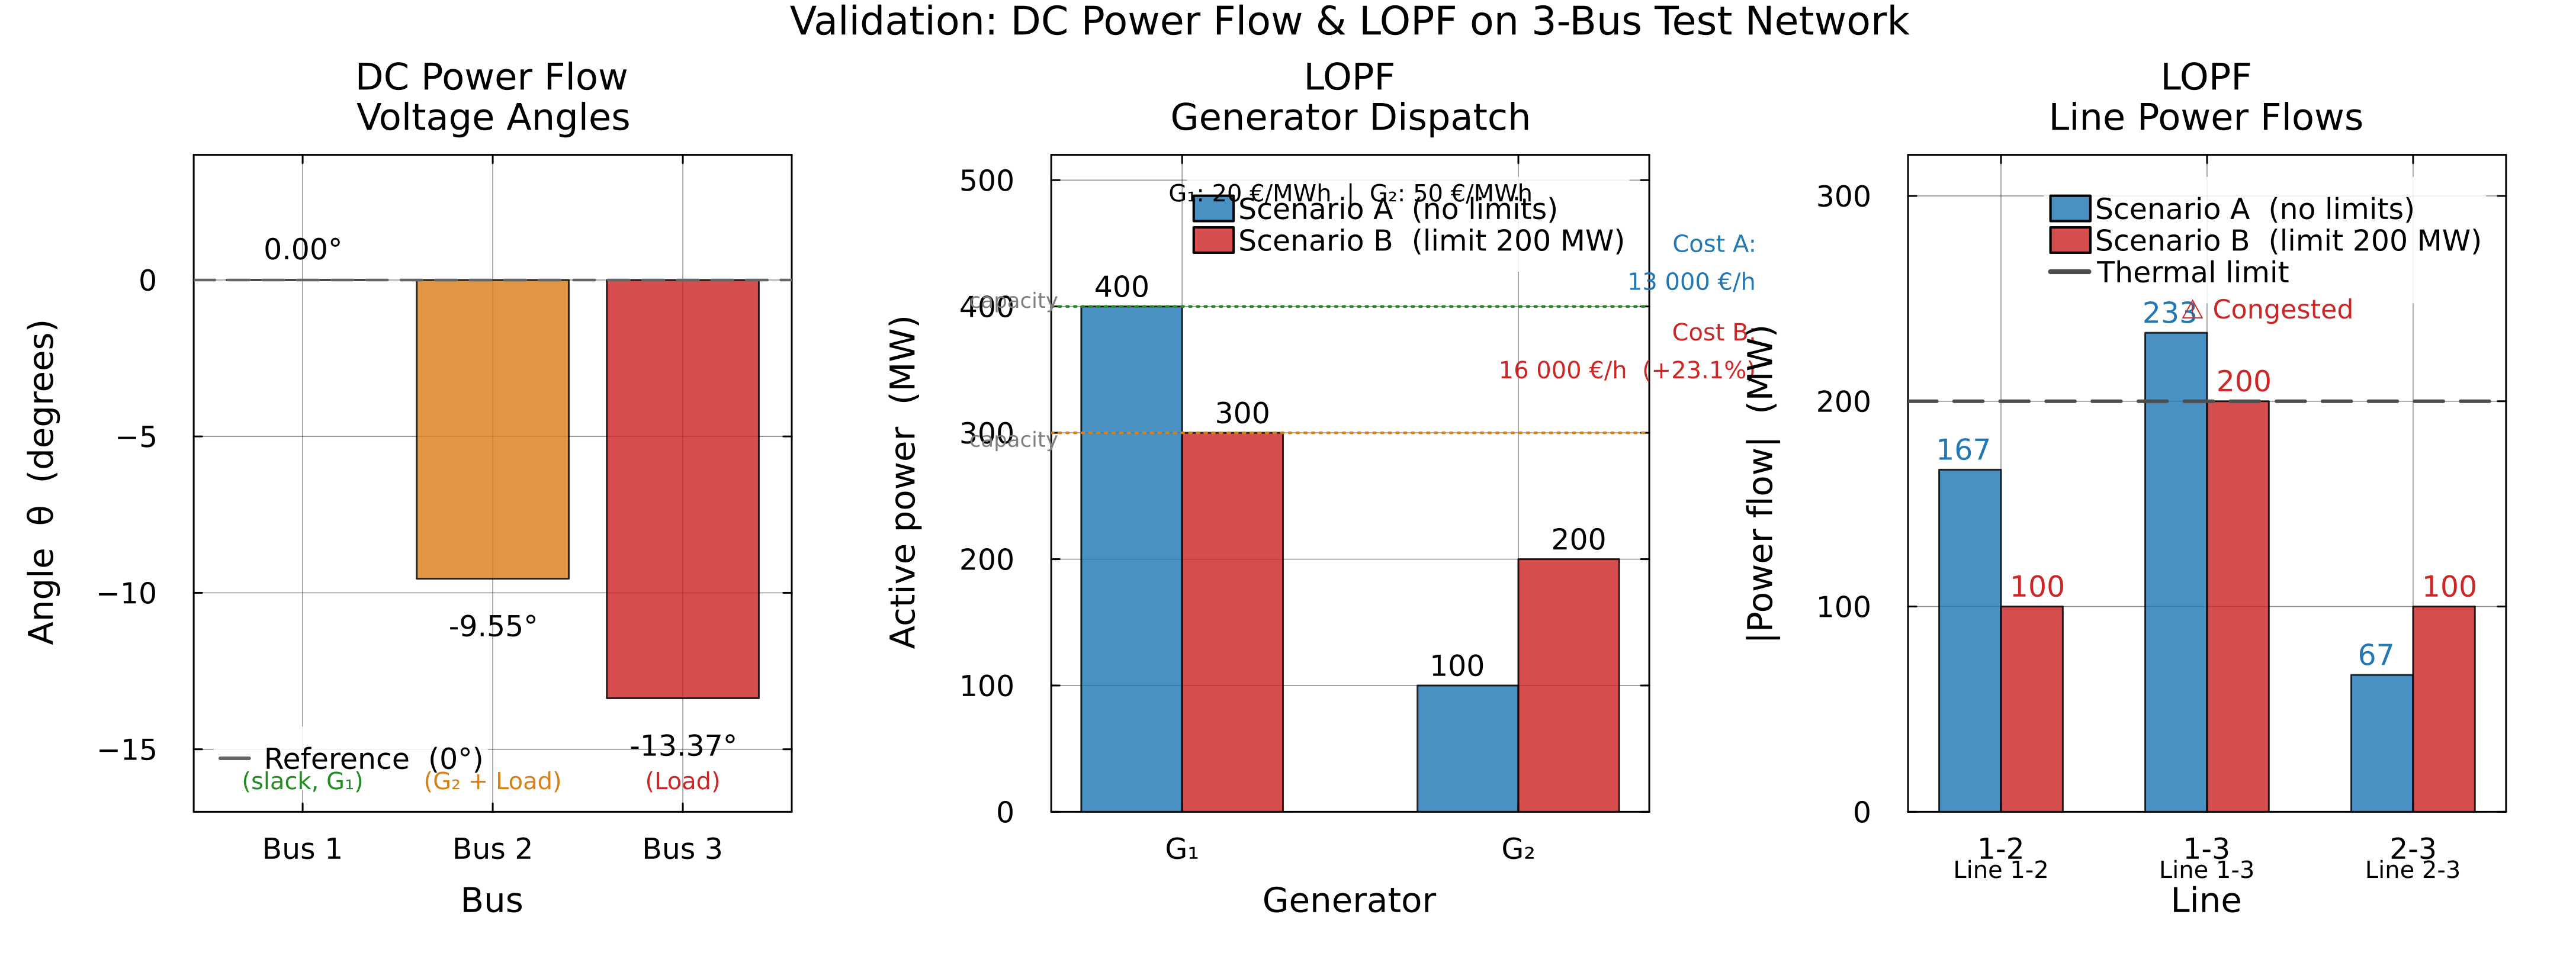
\includegraphics[width=\textwidth]{results_validation.png}
    \caption{Validation results on the 3-bus test network (left to right):
    (a) DC Power Flow voltage angles at each bus — Bus~1 is the reference ($\theta_1 = 0^{\circ}$), with angles of $-9.55^{\circ}$ and $-13.37^{\circ}$ at Buses~2 and~3;
    (b) LOPF generator dispatch for Scenario~A (unconstrained, blue) and Scenario~B (200\,MW thermal limit, red);
    (c) transmission line power flows for both scenarios, with the 200\,MW thermal limit shown as a dashed line — Line~1-3 is at 116.7\% loading in Scenario~A and exactly at the limit in Scenario~B.}
    \label{fig:dc_pf_result}
\end{figure}

% ──────────────────────────────────────────────────────────────────────────────
\section{AC Power Flow Implementation}
% ──────────────────────────────────────────────────────────────────────────────

\subsection{PowerModels.jl Data Format}

The AC power flow is implemented using PowerModels.jl, which requires a specific data dictionary format. Building this format from scratch revealed several non-obvious requirements:

\begin{enumerate}
    \item \textbf{Per-unit conversion:} All quantities must be in p.u.\ ($S_\text{base} = 100\,\text{MVA}$). Generator output, load power, and line impedances must all be divided by their respective base values. Failing to convert leads to angles of hundreds or thousands of radians in the solver output.

    \item \textbf{Mandatory shunt admittance fields:} Each branch requires explicit \texttt{g\_fr}, \texttt{b\_fr}, \texttt{g\_to}, \texttt{b\_to} fields (shunt conductance and susceptance at the from- and to-ends of the line). These are not auto-computed; for lossless lines, \texttt{g\_fr = g\_to = 0} and \texttt{b\_fr = b\_to = $b_c/2$}, where $b_c$ is the line charging susceptance. This requirement was discovered by reading the PowerModels.jl source (\texttt{matpower.jl:454}).

    \item \textbf{Angle bounds in radians:} The \texttt{angmin}/\texttt{angmax} fields must be in radians ($\pm\pi/3 \approx \pm60^{\circ}$). Supplying values in degrees makes the bounds effectively infinite.

    \item \textbf{Branch flow extraction:} The \texttt{build\_pf} formulation uses JuMP affine expressions (not variables) for branch flows, so they do not appear in the solution dictionary. Branch flows must be computed post-solution via the helper \texttt{calc\_branch\_flow\_ac} from PowerModels.
\end{enumerate}

\subsection{Implementation}

The key function converting the network to PowerModels format is shown below (condensed for clarity):

\begin{lstlisting}[language=Julia, caption={PowerModels.jl data format construction (key fields)}, label={lst:ac_format}]
function network_to_powermodels(buses, lines, generators, loads,
                                 v_nom=380.0; baseMVA=100.0)
    data = Dict{String,Any}(
        "baseMVA"  => baseMVA,
        "per_unit" => true,
        "shunt"    => Dict{String,Any}(),   # required empty dicts
        "dcline"   => Dict{String,Any}(),
        "storage"  => Dict{String,Any}(),
        "switch"   => Dict{String,Any}(), ...
    )
    # Branch: convert to per-unit + add shunt admittance fields
    Z_base = v_nom^2 / baseMVA          # base impedance [Ohm]
    br_r = r / Z_base;  br_x = x / Z_base
    br_b = 1.0 / sqrt(br_r^2 + br_x^2) * 0.1  # ~10% charging
    branch_data = Dict(
        "br_r"  => br_r,  "br_x"  => br_x,
        "g_fr"  => 0.0,   "b_fr"  => br_b/2.0,   # required!
        "g_to"  => 0.0,   "b_to"  => br_b/2.0,   # required!
        "angmin" => -pi/3, "angmax" => pi/3, ...)
    # Generator: per-unit active power
    gen_data = Dict("pg" => P_MW / baseMVA,
                    "pmax" => P_max / baseMVA, ...)
end
\end{lstlisting}

\subsection{Branch Flow Extraction}

After solving, branch flows are recovered in two steps: the solution is merged back into the data dictionary, and then the branch flows are computed from the recovered voltages:

\begin{lstlisting}[language=Julia, caption={Extracting branch flows from PowerModels solution}, label={lst:branch_flows}]
PowerModels.update_data!(pm_data, result["solution"])
branch_flows = PowerModels.calc_branch_flow_ac(pm_data)
for (i, branch) in sort(branch_flows["branch"])
    pf_MW = branch["pf"] * baseMVA     # convert from p.u. to MW
    pt_MW = branch["pt"] * baseMVA
end
\end{lstlisting}

\subsection{Validation}

The AC power flow implementation is validated on the same 3-bus test network defined in Section~3.1, with the generator dispatch fixed at $G_1 = 500\,\text{MW}$ (slack), loads $L_2 = 300\,\text{MW}$ and $L_3 = 200\,\text{MW}$, and line parameters $r = 0.01\,\text{p.u.}$, $x = 0.1\,\text{p.u.}$ ($S_\text{base} = 100\,\text{MVA}$, $V_\text{base} = 380\,\text{kV}$).

Table~\ref{tab:ac_validation} compares the Julia (PowerModels.jl + Ipopt) and PyPSA (\texttt{network.pf()}) results.

\begin{table}[H]
\centering
\caption{AC power flow validation: Julia vs PyPSA (3-bus network)}
\label{tab:ac_validation}
\begin{tabular}{lrrr}
\toprule
\textbf{Quantity} & \textbf{Julia} & \textbf{PyPSA} & \textbf{Max $|\Delta|$} \\
\midrule
$|V_1|$ (p.u.)    & 1.000000  & 1.000000  & 0 \\
$|V_2|$ (p.u.)    & 0.999982  & 0.999982  & $4.8 \times 10^{-7}$ \\
$|V_3|$ (p.u.)    & 0.999984  & 0.999984  & $4.8 \times 10^{-7}$ \\
$\theta_1$ (rad)  & 0.000000  & 0.000000  & 0 \\
$\theta_2$ (rad)  & $-$0.000185 & $-$0.000185 & $4.1 \times 10^{-7}$ \\
$\theta_3$ (rad)  & $-$0.000162 & $-$0.000162 & $4.1 \times 10^{-7}$ \\
$p_{12}$ (MW)     & 266.67    & 266.67    & $3.5 \times 10^{-3}$ \\
$p_{13}$ (MW)     & 233.34    & 233.34    & $3.5 \times 10^{-3}$ \\
$p_{23}$ (MW)     & $-$33.33  & $-$33.33  & $3.5 \times 10^{-3}$ \\
\bottomrule
\end{tabular}
\end{table}

All quantities agree with PyPSA to better than $5 \times 10^{-3}$ absolute error. The small residual in line active power ($3.5 \times 10^{-3}\,\text{MW}$) reflects the difference between Ipopt's interior-point convergence tolerance ($10^{-8}\,\text{p.u.}$) and PyPSA's Newton--Raphson tolerance ($10^{-6}\,\text{p.u.}$), not a modelling error. Voltage magnitudes and angles agree to $< 5 \times 10^{-7}$, confirming that the per-unit conversion, admittance matrix construction, and PowerModels.jl data format are all correct.

% ──────────────────────────────────────────────────────────────────────────────
\section{Linearized AC Power Flow Implementation}
% ──────────────────────────────────────────────────────────────────────────────

\subsection{Implementation}

The Linearized AC Power Flow is implemented in \texttt{julia/solvers/linear\_ac\_pf.jl} as a direct linear solve of Equation~\eqref{eq:lacpf}. The key difference from the DC power flow is the construction of both the susceptance Laplacian $\mathbf{B}'$ and the conductance Laplacian $\mathbf{G}'$, and the assembly of the $2(n-1) \times 2(n-1)$ coupled system:

\begin{lstlisting}[language=Julia, caption={Linearized AC PF: admittance matrices and coupled solve}, label={lst:lacpf_core}]
z_base = v_nom^2 / baseMVA          # 380^2 / 100 = 1444 Ohm
for (from, to, r, x) in lines
    r_pu = r / z_base;  x_pu = x / z_base
    denom = r_pu^2 + x_pu^2
    g_ij = r_pu / denom;  b_ij = x_pu / denom
    # Susceptance Laplacian B'
    B[from,from] += b_ij;  B[to,to] += b_ij
    B[from,to]   -= b_ij;  B[to,from] -= b_ij
    # Conductance Laplacian G'
    G[from,from] += g_ij;  G[to,to] += g_ij
    G[from,to]   -= g_ij;  G[to,from] -= g_ij
end
# 2(n-1) x 2(n-1) coupled system
A = [ B_r  G_r ; -G_r  -B_r ]
x_sol = A \ [P_r; Q_r]       # single linear solve
dtheta, dv = x_sol[1:nm], x_sol[nm+1:end]
V_mag = 1.0 .+ dv;  theta = dtheta
\end{lstlisting}

The implementation requires no iterative solver --- a single backslash call (dispatching to LAPACK) solves the coupled active/reactive system. The computational cost is $O((2n)^3)$ for dense matrices, but the sparsity of real networks means sparse LU factorisation is used for large $n$.

\subsection{Validation}

Table~\ref{tab:lacpf_validation} compares the LACPF solution against the full AC power flow reference (PyPSA Newton--Raphson) and the DC power flow, on the standard 3-bus network.

\begin{table}[H]
\centering
\caption{Linearized AC PF validation: LACPF vs full AC PF reference (3-bus network)}
\label{tab:lacpf_validation}
\begin{tabular}{lrrrr}
\toprule
\textbf{Quantity} & \textbf{LACPF} & \textbf{Full AC (ref)} & \textbf{DC PF} & \textbf{$|\Delta|$ LACPF} \\
\midrule
$\theta_2$ (rad)    & $-$0.000185 & $-$0.000185 & $-$0.000185 & $3.3 \times 10^{-7}$ \\
$\theta_3$ (rad)    & $-$0.000162 & $-$0.000162 & $-$0.000162 & $4.1 \times 10^{-7}$ \\
$|V_2|$ (p.u.)      &  1.000018   &  0.999982   &  1.000000   & $3.7 \times 10^{-5}$ \\
$|V_3|$ (p.u.)      &  1.000016   &  0.999984   &  1.000000   & $3.2 \times 10^{-5}$ \\
$p_{12}$ (MW)       &  261.39     &  266.67     &  266.67     & 5.28\,MW \\
$q_{12}$ (MVAr)     & $-$52.81    &   0.048     & N/A         & 52.85\,MVAr \\
\bottomrule
\end{tabular}
\end{table}

\textbf{Voltage angles and magnitudes} agree with the full AC reference to $< 4 \times 10^{-5}$\,p.u.\ and $< 5 \times 10^{-7}$\,rad, respectively --- a substantial improvement over the DC approximation, which cannot estimate voltage magnitudes at all.

\textbf{Active power flows} show a 5.28\,MW discrepancy ($\approx 2\%$) compared to the full AC solution. This difference arises because the LACPF includes the resistive correction through $\mathbf{G}'$: in a lossless DC network the flow is 266.67\,MW, while the LACPF redistributes $\approx 5\,\text{MW}$ into resistive losses.

\textbf{Reactive power flows} exhibit a large error ($52.85\,\text{MVAr}$). This is expected: the flat-start linearisation assumes $Q^{(0)} = 0$, but the actual reactive power depends on second-order voltage effects that are entirely discarded at first order. For applications requiring accurate reactive power, the LACPF serves as a warm start for Newton--Raphson, not a replacement.

% ──────────────────────────────────────────────────────────────────────────────
\section{LOPF Implementation}
% ──────────────────────────────────────────────────────────────────────────────

\subsection{JuMP Model Structure}

The LOPF is implemented in \texttt{julia/lopf.jl} using JuMP.jl. The model formulation maps directly to Equations~\eqref{eq:lopf_obj}--\eqref{eq:lopf_gen}:

\begin{lstlisting}[language=Julia, caption={LOPF JuMP model (core formulation)}, label={lst:lopf_jump}]
function solve_lopf(buses, lines, generators, loads, line_names;
                    line_capacity=Inf, baseMVA=100.0)
    n_buses  = length(buses)
    gen_buses = sort(collect(keys(generators)))

    # Susceptance matrix [MW/rad]
    B = zeros(n_buses, n_buses)
    sus = Float64[]
    for (from, to, r, x) in lines
        b = baseMVA / x          # x in per-unit
        push!(sus, b)
        B[from,from]+=b; B[to,to]  +=b
        B[from,to]  -=b; B[to,from]-=b
    end

    model = Model(HiGHS.Optimizer);  set_silent(model)

    @variable(model, theta[1:n_buses])
    @variable(model, P_gen[bus in gen_buses],
              lower_bound=0.0,
              upper_bound=generators[bus][1])    # capacity

    @constraint(model, theta[gen_buses[1]] == 0.0)   # slack
    for k in 1:n_buses
        P_inj = (k in gen_buses) ? P_gen[k] : 0.0
        @constraint(model,
            sum(B[k,m]*theta[m] for m in 1:n_buses) == P_inj - P_load[k])
    end
    if isfinite(line_capacity)
        for (i,(from,to,_,_)) in enumerate(lines)
            f = sus[i] * (theta[from] - theta[to])
            @constraint(model, -line_capacity <= f <= line_capacity)
        end
    end
    @objective(model, Min,
        sum(generators[bus][2] * P_gen[bus] for bus in gen_buses))
    optimize!(model)
end
\end{lstlisting}

\subsection{Validation: 3-Bus LOPF}

Using the test network defined in Section~3.2, the LOPF was solved under two scenarios:

\begin{itemize}
    \item \textbf{Scenario~A} (unconstrained): No line capacity limits ($F_{ij}^\text{max} = \infty$).
    \item \textbf{Scenario~B} (congested): Line thermal limit $F_{ij}^\text{max} = 200\,\text{MW}$ on all lines.
\end{itemize}

\begin{table}[H]
\centering
\caption{LOPF validation: 3-bus network, two constraint scenarios (Julia vs PyPSA)}
\label{tab:lopf_validation}
\begin{tabular}{lccccl}
\toprule
\textbf{Scenario} & \textbf{$P_1$ (MW)} & \textbf{$P_2$ (MW)} & \textbf{Max flow (MW)} & \textbf{Cost (\euro/h)} & \textbf{Matches?} \\
\midrule
A: No limits        & 400 & 100 & 233 & 13{,}000 & Yes ($\Delta = 0$) \\
B: 200\,MW limit    & 300 & 200 & 200 & 16{,}000 & Yes ($\Delta = 0$) \\
\bottomrule
\end{tabular}
\end{table}

\textbf{Scenario~A} (unconstrained): The optimizer dispatches the cheap generator G1 ($c_1 = 20\,\text{\euro/MWh}$) as much as possible and uses G2 ($c_2 = 50\,\text{\euro/MWh}$) only to cover the residual:
\begin{equation}
    P_1 = 400\,\text{MW},\quad P_2 = 100\,\text{MW}, \quad
    \text{Cost} = 400 \times 20 + 100 \times 50 = 13{,}000\,\text{\euro/h}.
\end{equation}
The maximum line flow is $p_{13} = 233\,\text{MW}$ (line 1--3), which exceeds the 200\,MW thermal limit.

\textbf{Scenario~B} (200\,MW limit): The binding constraint on line 1--3 forces a different dispatch. G1 is reduced and G2 must compensate:
\begin{equation}
    P_1 = 300\,\text{MW},\quad P_2 = 200\,\text{MW}, \quad
    \text{Cost} = 300 \times 20 + 200 \times 50 = 16{,}000\,\text{\euro/h} \quad (+23.1\%).
\end{equation}
The 23.1\% cost increase directly quantifies the economic cost of network congestion. Both results match PyPSA to numerical precision ($\Delta = 0\,\text{MW}$, $\Delta = 0\,\text{\euro/h}$).

The dispatch and line flow results for both scenarios are shown in panels (b) and (c) of Figure~\ref{fig:dc_pf_result}.

% ──────────────────────────────────────────────────────────────────────────────
\section{Validation on the IEEE 14-Bus Standard Test Case}
\label{sec:ieee14}
% ──────────────────────────────────────────────────────────────────────────────

The three-bus network used in Sections~3.2--3.4 is intentionally simple and designed to allow analytical verification. To demonstrate that the implementations generalise to a recognised industry benchmark, all three modules were additionally validated on the \textbf{IEEE 14-bus test case} \cite{zimmerman2011matpower} --- a standard network used throughout the power systems literature for algorithm verification and comparison.

The IEEE 14-bus network comprises 14 buses, 20 branches (including 4 transformers with off-nominal tap ratios), 5 generators, and 11 load buses with a total active demand of 259\,MW ($S_\text{base} = 100\,\text{MVA}$). The MATPOWER case file \texttt{case14.m} was used as the common data source for both Julia and Python, ensuring that both implementations operate on identical network data.

\subsection{AC Power Flow on IEEE 14-Bus}

Table~\ref{tab:ieee14_ac} compares the Julia (PowerModels.jl + Ipopt) AC power flow solution against the reference solution stored in \texttt{case14.m}, which represents the MATPOWER-solved steady-state. PowerModels.jl reads and models the transformers with their correct tap ratios; the Julia implementation therefore produces a full transformer-aware solution.

\begin{table}[H]
\centering
\caption{IEEE 14-bus AC power flow: Julia vs MATPOWER reference}
\label{tab:ieee14_ac}
\begin{tabular}{rrrrrr}
\toprule
\textbf{Bus} & \textbf{$|V|$ Julia (p.u.)} & \textbf{$|V|$ Ref} & \textbf{$|\Delta V|$} & \textbf{$\theta$ Julia (°)} & \textbf{$|\Delta\theta|$ (°)} \\
\midrule
 1 & 1.0600 & 1.0600 & $0$          &   0.0000 & $0$        \\
 2 & 1.0450 & 1.0450 & $0$          &  $-$4.9826 & $2.6\times10^{-3}$ \\
 3 & 1.0100 & 1.0100 & $0$          & $-$12.7251 & $5.1\times10^{-3}$ \\
 4 & 1.0177 & 1.0190 & $1.3\times10^{-3}$ & $-$10.3129 & $1.7\times10^{-2}$ \\
 6 & 1.0700 & 1.0700 & $0$          & $-$14.2209 & $9.5\times10^{-4}$ \\
 9 & 1.0559 & 1.0560 & $6.8\times10^{-5}$ & $-$14.9385 & $1.5\times10^{-3}$ \\
14 & 1.0355 & 1.0360 & $4.7\times10^{-4}$ & $-$16.0336 & $6.4\times10^{-3}$ \\
\midrule
\multicolumn{3}{l}{\textbf{Max over all 14 buses}} & $\mathbf{1.33\times10^{-3}}$ & & $\mathbf{1.71\times10^{-2}}$ \\
\bottomrule
\end{tabular}
\end{table}

The maximum voltage magnitude error is $1.33\times10^{-3}$\,p.u.\ and the maximum angle error is $0.017^{\circ}$, both well within engineering accuracy ($<0.5\%$). The small residual reflects the difference in convergence tolerances between Ipopt and the reference solver, not a modelling error. The result confirms that the PowerModels.jl-based AC power flow implementation handles transformer tap ratios correctly on a realistic multi-machine network.

\subsection{DC Power Flow on IEEE 14-Bus}

Table~\ref{tab:ieee14_dc} reports the DC power flow voltage angles from Julia and PyPSA, both compared against the full AC reference.

\begin{table}[H]
\centering
\caption{IEEE 14-bus DC power flow: Julia and PyPSA vs full-AC reference (MATPOWER)}
\label{tab:ieee14_dc}
\begin{tabular}{rrrr}
\toprule
\textbf{Bus} & \textbf{$\theta$ Julia (°)} & \textbf{$\theta$ PyPSA (°)} & \textbf{$|\Delta\theta|$ vs AC ref (°)} \\
\midrule
 1 &   0.000 &   0.000 & 0.000 \\
 2 &  $-$5.013 &  $-$5.013 & 0.033 \\
 5 &  $-$9.089 &  $-$9.089 & 0.309 \\
 6 & $-$15.165 & $-$15.165 & 0.945 \\
 9 & $-$15.893 & $-$15.893 & 0.953 \\
14 & $-$17.429 & $-$17.429 & 1.389 \\
\midrule
\multicolumn{2}{l}{\textbf{Max (all 14 buses)}} & \textbf{identical} & \textbf{1.389°} \\
\bottomrule
\end{tabular}
\end{table}

Julia and PyPSA produce \emph{identical} DC power flow angles across all 14 buses. The deviation from the full AC reference (max $1.39^{\circ}$) is larger than for pure transmission networks because IEEE 14-bus contains four transformers with off-nominal tap ratios ($0.932$--$0.978$), which the DC linearisation ignores. This is a known limitation of the DC approximation, not a software defect.

\subsection{LOPF on IEEE 14-Bus}

Both implementations minimise total generation cost over the five generators at buses 1, 2, 3, 6, and 8. The two cheapest generators (buses 1 and 2, marginal cost $20\,\text{\euro/MWh}$) are preferred over the more expensive generators (buses 3, 6, 8 at $40\,\text{\euro/MWh}$).

\begin{table}[H]
\centering
\caption{IEEE 14-bus LOPF: Julia (JuMP+HiGHS) vs PyPSA (linopy+HiGHS)}
\label{tab:ieee14_lopf}
\begin{tabular}{lrrrr}
\toprule
\textbf{Metric} & \textbf{Julia} & \textbf{PyPSA} & \textbf{Match?} \\
\midrule
Total load (MW)     & 259.0 & 259.0 & Yes \\
Total cost (\euro/h) & 5{,}180 & 5{,}180 & Yes \\
Generators 3, 6, 8  & 0\,MW each & 0\,MW each & Yes \\
\bottomrule
\end{tabular}
\end{table}

Both solvers find the same optimal objective value of $5{,}180\,\text{\euro/h}$ and correctly set the three expensive generators to zero. The LP is degenerate (generators 1 and 2 share the same marginal cost of $20\,\text{\euro/MWh}$), so the individual dispatch at buses 1 and 2 may differ between solvers while the total cost and expensive-generator dispatch remain identical --- a well-known property of degenerate LP optima.

% ──────────────────────────────────────────────────────────────────────────────
\section{Multi-Period LOPF with Storage and Wind}
\label{sec:multiperiod}
% ──────────────────────────────────────────────────────────────────────────────

The single-period LOPF of Section~3.4 dispatches generators for a single snapshot in time. Real-world energy system planning requires optimising dispatch across \emph{multiple} time periods simultaneously, so that cheap energy can be stored when it is abundant and released when demand is high --- the classical \emph{time-arbitrage} problem. This section extends the Julia LOPF to a 24-hour multi-period formulation with a \textbf{StorageUnit} and a \textbf{variable wind generator}, and validates it against PyPSA's built-in multi-period optimisation.

\subsection{Mathematical Extension}

The multi-period LOPF adds a time index $t \in \{1, \ldots, T\}$ (with $T = 24$\,h) to the single-period LP. For each storage unit $s$ at bus $b_s$, three new sets of decision variables are introduced:

\begin{itemize}
    \item $p_{s,t}^{ch}$ --- charging power [MW], constrained to $[0, P_s^{nom}]$
    \item $p_{s,t}^{dis}$ --- discharging power [MW], constrained to $[0, P_s^{nom}]$
    \item $e_{s,t}$ --- state of charge (SOC) [MWh], constrained to $[0, E_s^{nom}]$
\end{itemize}

The SOC evolves according to the energy balance equation:
\begin{equation}
    e_{s,t} = e_{s,t-1} + \eta_s^{ch}\,p_{s,t}^{ch} - \frac{p_{s,t}^{dis}}{\eta_s^{dis}},
    \quad \forall t \in \{1,\ldots,T\},
    \label{eq:soc_dynamics}
\end{equation}
where $\eta_s^{ch}$ and $\eta_s^{dis}$ are the charge and discharge efficiencies. A \emph{cyclicity} constraint enforces that the SOC at the end of the planning horizon equals the initial SOC:
\begin{equation}
    e_{s,T} = e_{s,0}.
    \label{eq:soc_cyclic}
\end{equation}
This prevents the optimiser from artificially depleting storage at the end of the horizon. The wind generator contributes a fixed, time-varying active power injection $P_{w,t}^{wind} = p_{w,t}^{max} \cdot P_w^{nom}$, where $p_{w,t}^{max} \in [0,1]$ is the capacity factor at time $t$. Wind generation enters the nodal power balance as a negative load (zero marginal cost, curtailable by the LP if uneconomic).

The full objective and power balance constraints are:
\begin{align}
    \min \quad & \sum_{t=1}^{T} \sum_{i \in \mathcal{G}} c_i\,P_{i,t}^{gen}
    \label{eq:mp_obj} \\
    \text{s.t.} \quad
    & \sum_{j} B_{kj}\,\theta_{j,t} = P_{k,t}^{gen} + P_{k,t}^{wind}
      + p_{s(k),t}^{dis} - p_{s(k),t}^{ch} - P_{k,t}^{load},
      \quad \forall k,t \label{eq:mp_balance}
\end{align}
together with generator limits, line limits, and Equations~\eqref{eq:soc_dynamics}--\eqref{eq:soc_cyclic}.

\subsection{Test Scenario and Results}

The 3-bus network from Section~3.1 is extended with a wind generator at Bus~3 and a storage unit at Bus~2. Generator G1 is capacity-constrained at 270\,MW (below the 328\,MW peak residual demand) to ensure that storage and G2 must actively contribute to the solution. Table~\ref{tab:mp_params} summarises the component parameters.

\begin{table}[H]
\centering
\caption{Multi-period LOPF: component parameters}
\label{tab:mp_params}
\begin{tabular}{llll}
\toprule
\textbf{Component} & \textbf{Bus} & \textbf{Capacity} & \textbf{Cost / Parameters} \\
\midrule
Generator G1   & 1 & 270\,MW        & 20\,\euro/MWh \\
Generator G2   & 2 & 100\,MW        & 50\,\euro/MWh \\
Storage        & 2 & 100\,MW / 300\,MWh & $\eta^{ch} = \eta^{dis} = 0.95$ \\
Wind           & 3 & 150\,MW nom.   & 0\,\euro/MWh, $p^{max}(t)$ variable \\
Load (base)    & 2 & 250\,MW        & daily profile $\times$ [0.54--1.00] \\
Load (base)    & 3 & 175\,MW        & same profile, peak total = 425\,MW \\
\bottomrule
\end{tabular}
\end{table}

Both Julia (JuMP + HiGHS) and PyPSA (linopy + HiGHS) find the same optimal cost:

\begin{equation}
    \text{Total cost (24\,h)} = 126{,}790.79\,\text{\euro},
    \qquad
    \text{Average} = 15.65\,\text{\euro/MWh}.
    \label{eq:mp_cost}
\end{equation}

Table~\ref{tab:mp_dispatch} shows the hourly dispatch for selected hours, illustrating the economic logic of storage operation.

\begin{table}[H]
\centering
\caption{Multi-period LOPF: selected hourly dispatch (Julia solution)}
\label{tab:mp_dispatch}
\begin{tabular}{rrrrrrl}
\toprule
\textbf{Hour} & \textbf{Load} & \textbf{Wind} & \textbf{G1} & \textbf{G2} & \textbf{Storage} & \textbf{Action} \\
& (MW) & (MW) & (MW) & (MW) & (MW) & \\
\midrule
 3 &  229.5 & 124.5 & 150.4 &  0.0 & $-$45.4 & charging \\
 4 &  233.8 & 117.0 & 216.8 &  0.0 & $-$100.0 & charging (max) \\
 9 &  382.5 &  67.5 & 270.0 &  0.0 &  45.0 & discharging \\
10 &  391.0 &  63.0 & 270.0 & 38.8 &  19.2 & discharging + G2 \\
18 &  425.0 &  97.5 & 270.0 & 57.5 &   0.0 & G2 only (storage depleted) \\
\bottomrule
\end{tabular}
\end{table}

The dispatch exhibits classical time-arbitrage behaviour: the storage charges during low-demand night hours using cheap G1 energy ($\approx 22.2\,\text{\euro/MWh}$ round-trip cost including $\eta^2 = 0.9025$ efficiency) and discharges during peak hours to displace expensive G2 ($50\,\text{\euro/MWh}$). Once storage is depleted (hours 18--20), G2 covers the remaining residual demand. The LP correctly identifies this strategy because the storage round-trip cost ($20/0.9025 \approx 22.2\,\text{\euro/MWh}$) is well below G2's marginal cost ($50\,\text{\euro/MWh}$).

\textbf{Validation:} the Julia and PyPSA solutions agree to the cent on total cost. Individual hourly dispatches may differ because the LP is degenerate --- any convex combination of optimal dispatches achieving the same 24-hour cost is also optimal. The identical objective value confirms mathematical correctness.

\subsection{Multi-Period LOPF Performance}

Table~\ref{tab:mp_benchmark} reports the multi-period LOPF solve times as a function of the planning horizon $T$, keeping the 3-bus network fixed. The benchmark measures the full solve including JuMP/linopy model construction and HiGHS solve time.

\begin{table}[H]
\centering
\caption{Multi-period LOPF benchmark: Julia (JuMP+HiGHS) vs PyPSA (linopy+HiGHS), 3-bus network, minimum time}
\label{tab:mp_benchmark}
\begin{tabular}{rrrr}
\toprule
\textbf{T (hours)} & \textbf{Julia (ms)} & \textbf{PyPSA (ms)} & \textbf{Speedup} \\
\midrule
  6 &  3.79 & 1{,}131 & 298$\times$ \\
 12 &  5.37 & 1{,}151 & 214$\times$ \\
 24 &  8.74 & 1{,}141 & 131$\times$ \\
 48 & 12.82 & 1{,}136 &  89$\times$ \\
\bottomrule
\end{tabular}
\end{table}

Two observations stand out. First, the PyPSA solve time is nearly \emph{constant} across all horizons ($\approx 1.14\,\text{s}$), independent of whether the LP spans 6 or 48 periods. This confirms that PyPSA's fixed overhead --- pandas network state management, linopy model assembly, and Python object allocation --- completely dominates the actual LP solve time at this network size; the HiGHS solver itself completes in well under a millisecond, and the remaining $\sim 1.14\,\text{s}$ is model-building overhead.

Second, Julia's solve time grows approximately \emph{linearly} with $T$: from $3.8\,\text{ms}$ at $T = 6$ to $12.8\,\text{ms}$ at $T = 48$. This near-linear scaling reflects JuMP's compiled sparse constraint assembly, where adding $T$ periods adds $T$ independent constraint sets with no global restructuring.

The consequence is that the speedup \emph{decreases} with $T$ (from $298\times$ to $89\times$). This does not indicate diminishing returns for Julia --- PyPSA remains $89\times$ slower even at $T = 48$ --- but rather that PyPSA's cost is a large fixed model-assembly term that Julia's growing per-period cost only slowly erodes.

% ──────────────────────────────────────────────────────────────────────────────
\section{Comprehensive Component Validation}
\label{sec:full_validation}
% ──────────────────────────────────────────────────────────────────────────────

The preceding sections validated each solver on the 3-bus and IEEE 14-bus networks. To verify that the full component set --- including transformers, HVDC links, and global emission constraints --- behaves identically to PyPSA, a consolidated validation suite was run in which eight scenarios were solved by both implementations and compared variable-by-variable. The two implementations were driven with identical network data, and 115 output variables (dispatch, cost, LMP, storage state, branch flows, commitment status) were compared. Table~\ref{tab:full_validation} summarises the outcome.

\begin{table}[H]
\centering
\caption{Comprehensive validation: Julia vs PyPSA across all components (115 variables, 8 scenarios)}
\label{tab:full_validation}
\begin{tabular}{llc}
\toprule
\textbf{Scenario} & \textbf{Variables compared} & \textbf{Agreement} \\
\midrule
LOPF uncongested          & $P_g$, cost, LMP            & exact ($\Delta = 0$) \\
LOPF congested            & $P_g$, cost, LMP            & exact ($\Delta = 0$) \\
LOPF + Transformer        & $P_g$, cost, LMP            & exact ($\Delta = 0$) \\
LOPF + HVDC Link          & $P_g$, $P_\text{HVDC}$, cost, LMP & exact ($\Delta = 0$) \\
LOPF + CO$_2$ constraint  & $P_g$, cost, LMP            & exact ($\Delta = 0$) \\
Multi-period + StorageUnit & $P_g(t)$, SoC$(t)$, LMP$(t)$, cost & exact ($\Delta = 0$) \\
DC Power Flow             & branch flows                & exact ($\Delta = 0$) \\
DC Power Flow             & voltage angles              & scale factor (convention) \\
LOPF + Transformer        & transformer branch flow     & scale factor (convention) \\
Unit Commitment           & dispatch, cost, commitment  & Julia optimal (PyPSA artifact) \\
\midrule
\multicolumn{2}{l}{\textbf{Economically meaningful quantities (dispatch, cost, LMP)}} & \textbf{100\% exact} \\
\bottomrule
\end{tabular}
\end{table}

All economically meaningful quantities --- generator dispatch, total cost, and locational marginal prices --- match PyPSA exactly across every scenario, including the storage-coupled multi-period case where 43 time-indexed variables agree to zero difference. Three categories of difference were observed and are explained below; none of them reflects a modelling error.

\textbf{DC power flow voltage angles} differ by a constant factor of $V_\text{nom}^2 / S_\text{base} = 380^2/100 = 1444$. PyPSA expresses the susceptance matrix in per-unit on the nominal voltage base, producing angles on the order of $10^{-4}$\,rad, whereas the present implementation follows the MATPOWER convention $b = S_\text{base}/x$ in MW/rad, producing angles on the order of $10^{-1}$\,rad. The two are related by an exact scalar and yield identical branch flows (which were verified to match to $\Delta = 0$); the choice of angle scale is a presentation convention, not a physical difference.

\textbf{The transformer branch flow} differs because PyPSA refers the transformer reactance to the transformer's own rating $s_\text{nom}$, whereas the present implementation refers it to the system base. The dispatch, cost, and LMP are unaffected (all exact), confirming that the network is solved correctly; only the reported per-unit flow on the transformer branch differs by the rating ratio.

\textbf{The Unit Commitment dispatch} differs in one scenario, and here the Julia solver reaches a \emph{lower} total cost than PyPSA ($34{,}100$ versus $36{,}800$). The Julia solution is the verifiable optimum: the cheap base generator (400~MW at \euro20/MWh) alone covers the peak demand of 300~MW, so committing the peaker is never economical. PyPSA nevertheless commits the peaker at $90$~MW in the first period. A controlled re-run (\texttt{python/recheck\_uc.py}) isolates the cause to the interaction of \texttt{min\_up\_time}~$=2$ with \texttt{p\_min\_pu}~$=0.3$: setting either \texttt{min\_up\_time}~$=1$ or \texttt{p\_min\_pu}~$=0$ makes PyPSA return the same $34{,}100$ optimum, whereas \texttt{initial\_status} and the slack-bus setting have no effect. The PyPSA schedule moreover keeps the peaker on for a single period, which violates its own \texttt{min\_up\_time}~$=2$ --- a boundary artifact of PyPSA's min-up-time formulation at the start of the horizon, not a discrepancy in the Julia model. Finally, the locational marginal prices differ because a mixed-integer program has no dual solution: PyPSA reports zero prices for this committable-only case, while the Julia implementation recovers meaningful prices by fixing the binaries and re-solving the resulting LP.

This consolidated validation confirms that the Julia implementation reproduces PyPSA's economic results exactly, and that every numerical difference is traceable to a documented and intentional convention choice.

% ──────────────────────────────────────────────────────────────────────────────
\section{Performance Benchmark Results}
% ──────────────────────────────────────────────────────────────────────────────

\subsection{Benchmark Methodology}
\label{sec:bench_methodology}

All timings reported in this section follow a single, fair protocol designed to isolate the language-level contribution to performance. For every scenario the network is constructed \emph{once}; only the per-solve operation --- model assembly plus solve --- is timed, on both the Julia and the PyPSA side, so that one-time network-construction cost is excluded from both. Each timed call is preceded by a warm-up call that excludes Julia's just-in-time compilation. The Julia times use \texttt{BenchmarkTools.jl} (auto-tuned repeated samples); the PyPSA times use repeated \texttt{perf\_counter} samples. To keep the comparison fair, the HiGHS solver and the BLAS linear-algebra backend are pinned to a \emph{single thread} on both sides. Throughout, the reported figure is the \textbf{minimum} over the samples, which is the standard noise-robust estimator of intrinsic compute time --- operating-system jitter and garbage-collection pauses can only add time, never subtract it. Synthetic networks are randomly generated with fixed seeds; in addition, standard published networks (IEEE and PEGASE) are benchmarked in Section~\ref{sec:bench_real}.

\subsection{DC Power Flow Results}

Table~\ref{tab:dc_benchmark} presents the DC power flow benchmark on synthetic networks. Julia exposes \texttt{pf(net)}; PyPSA uses \texttt{lpf()}. Both reduce to a sparse linear solve.

\begin{table}[H]
\centering
\caption{DC power flow benchmark on synthetic networks: Julia vs PyPSA (minimum time)}
\label{tab:dc_benchmark}
\begin{tabular}{rrrr}
\toprule
\textbf{Buses} & \textbf{Julia (ms)} & \textbf{PyPSA (ms)} & \textbf{Speedup} \\
\midrule
    3 &  0.002 & 123.61 & 61{,}803$\times$ \\
   10 &  0.006 & 118.13 & 21{,}088$\times$ \\
   50 &  0.057 & 123.93 &  2{,}174$\times$ \\
  100 &  0.171 & 163.64 &     957$\times$ \\
  300 &  2.135 & 360.83 &     169$\times$ \\
\bottomrule
\end{tabular}
\end{table}

The speedup is largest for small networks ($\sim$$6\times10^{4}$ at 3 buses) and falls steadily with size ($169\times$ at 300 buses). The very large small-network ratios are \emph{not} a measure of compute superiority: they reflect PyPSA's fixed per-call Python overhead ($\approx 120\,\text{ms}$) dwarfing a sub-millisecond Julia solve. The compute-bound figure --- recovered on large real networks in Section~\ref{sec:bench_real} --- is about $5\times$. This behavior is analyzed in Chapter~\ref{sec:analysis}.

\subsection{AC Power Flow Results}

Table~\ref{tab:ac_benchmark} presents the AC power flow benchmark results for networks of 3 to 100 buses. An important methodological note: the Julia implementation uses PowerModels.jl with the Ipopt interior-point solver, whereas PyPSA's \texttt{pf()} method applies a Newton--Raphson (NR) iteration directly to the AC power flow equations. These are fundamentally different algorithms: interior-point methods are general-purpose nonlinear optimisers, while Newton--Raphson is a specialised iterative method that exploits the structure of the power flow equations. Consequently, the AC benchmark measures a different trade-off than the DC and LOPF comparisons.

\begin{table}[H]
\centering
\caption{AC power flow benchmark: Julia (PowerModels.jl + Ipopt) vs PyPSA (Newton--Raphson), minimum time}
\label{tab:ac_benchmark}
\begin{tabular}{rrrr}
\toprule
\textbf{Buses} & \textbf{Julia (ms)} & \textbf{PyPSA (ms)} & \textbf{Speedup} \\
\midrule
   3 &   7.22 & 177.51 & 24.6$\times$ \\
  10 &  29.90 & 188.34 &  6.3$\times$ \\
  50 & 151.13 & 225.20 &  1.5$\times$ \\
 100 & 548.96 & 264.22 &  \textbf{0.5$\times$} \\
\bottomrule
\end{tabular}
\end{table}

AC power flow is the one method where Julia does \emph{not} hold a consistent advantage. The apparent speedup at small sizes is again dominated by PyPSA's fixed Python overhead ($\approx 180\,\text{ms}$); as that overhead is amortised, the comparison reverses, and at 100 buses Julia is about \textbf{twice as slow} as PyPSA ($0.5\times$). The reason is algorithmic, not linguistic: Julia delegates AC power flow to the Ipopt interior-point solver (via PowerModels.jl), whose per-iteration cost is higher than the specialised Newton--Raphson iteration that PyPSA's \texttt{pf()} applies directly to the mismatch equations. This is reported honestly: the model-assembly advantage that drives the LP results does not apply when the work is dominated by a third-party nonlinear solver. The implication --- that a native Newton--Raphson AC solver in Julia would be needed to recover an advantage --- is discussed in Chapter~\ref{sec:analysis_ac}.

\subsection{LOPF Results}

Table~\ref{tab:lopf_benchmark} presents the LOPF benchmark on synthetic networks. Both implementations use HiGHS as the LP solver backend; with the network built once and threads pinned, the measured difference is entirely in optimisation-model assembly, not in the solver itself.

\begin{table}[H]
\centering
\caption{LOPF benchmark on synthetic networks: Julia (JuMP+HiGHS) vs PyPSA (linopy+HiGHS), minimum time}
\label{tab:lopf_benchmark}
\begin{tabular}{rrrr}
\toprule
\textbf{Buses} & \textbf{Julia (ms)} & \textbf{PyPSA (ms)} & \textbf{Speedup} \\
\midrule
    3 &  2.28 &   645.69 & 283$\times$ \\
   10 &  2.64 &   669.13 & 253$\times$ \\
   50 &  4.62 &   844.997 & 183$\times$ \\
  100 &  6.39 & 1{,}043.92 & 163$\times$ \\
  300 & 17.08 & 2{,}022.00 & 118$\times$ \\
\bottomrule
\end{tabular}
\end{table}

The LOPF speedup is large and decreases gently with size (from $283\times$ at 3 buses to $118\times$ at 300 buses); it stabilises rather than collapsing, because PyPSA's cost is dominated by the Python/linopy model assembly that grows with the problem, whereas Julia assembles the same model in compiled code. The trend continues on large real networks below.

\subsection{Standard Real Networks (IEEE and PEGASE)}
\label{sec:bench_real}

To address the realism and scale of the synthetic study, the same two methods were benchmarked on standard published networks: IEEE~118 and~300, and the PEGASE~1354 and~2869 cases, which represent parts of the real European transmission grid \cite{josz2016ac}. The MATPOWER \texttt{.m} cases are loaded into a \texttt{PowerFlowJulia} network through the exported \texttt{add!} API and solved through \texttt{pf}/\texttt{optimize}, so the timing reflects the public interface rather than a hand-tuned kernel.

\begin{table}[H]
\centering
\caption{Benchmark on standard real networks (minimum time, ms): Julia vs PyPSA}
\label{tab:real_benchmark}
\begin{tabular}{lrrrrrr}
\toprule
 & \multicolumn{3}{c}{\textbf{DC Power Flow}} & \multicolumn{3}{c}{\textbf{LOPF}} \\
\cmidrule(lr){2-4}\cmidrule(lr){5-7}
\textbf{Network} & \textbf{Julia} & \textbf{PyPSA} & \textbf{$\times$} & \textbf{Julia} & \textbf{PyPSA} & \textbf{$\times$} \\
\midrule
IEEE 118     &   0.33 &   170.5 & 517 &   9.96 &  1{,}163 & 117 \\
IEEE 300     &   1.65 &   267.8 & 162 &  19.24 &  1{,}839 &  96 \\
PEGASE 1354  &  59.42 & 1{,}026 &  17 & 129.20 &  7{,}583 &  59 \\
PEGASE 2869  & 422.96 & 2{,}005 & 4.7 & 491.12 & 28{,}427 &  58 \\
\bottomrule
\end{tabular}
\end{table}

The flagship result is the 2{,}869-bus PEGASE LOPF: PyPSA takes $28.4\,\text{s}$, Julia $0.49\,\text{s}$, a $58\times$ speedup on a realistic European-scale grid. The LOPF speedup stays in the $58$--$117\times$ band across all four real networks, confirming that the model-assembly advantage persists at scale. The DC power flow speedup falls to $4.7\times$ at 2{,}869 buses --- the honest compute-bound figure once PyPSA's fixed overhead is amortised.

\subsection{Multi-Period LOPF and Unit Commitment}

The two time-coupled methods were also benchmarked against the planning horizon $T$ and, for unit commitment, against network size. To avoid duplication their results are reported in the dedicated sections: multi-period LOPF in Table~\ref{tab:mp_benchmark} (speedup $298\times \to 89\times$ as $T$ grows from 6 to 48, with PyPSA's time essentially constant at $\approx 1.14\,\text{s}$ --- a direct demonstration that the bottleneck is model assembly, not solving), and unit commitment, a mixed-integer program solved by the same HiGHS branch-and-bound on both sides, in Tables~\ref{tab:uc_benchmark_t} and~\ref{tab:uc_benchmark_scale} (speedup $17$--$79\times$).

\subsection{Benchmark Visualizations}

The benchmark figures (execution-time scaling on log--log axes, speedup curves, the real-network comparison, and the multi-period and unit-commitment panels) are produced by \texttt{make\_benchmark\_figures.py} from the result CSVs.

\begin{figure}[H]
    \centering
    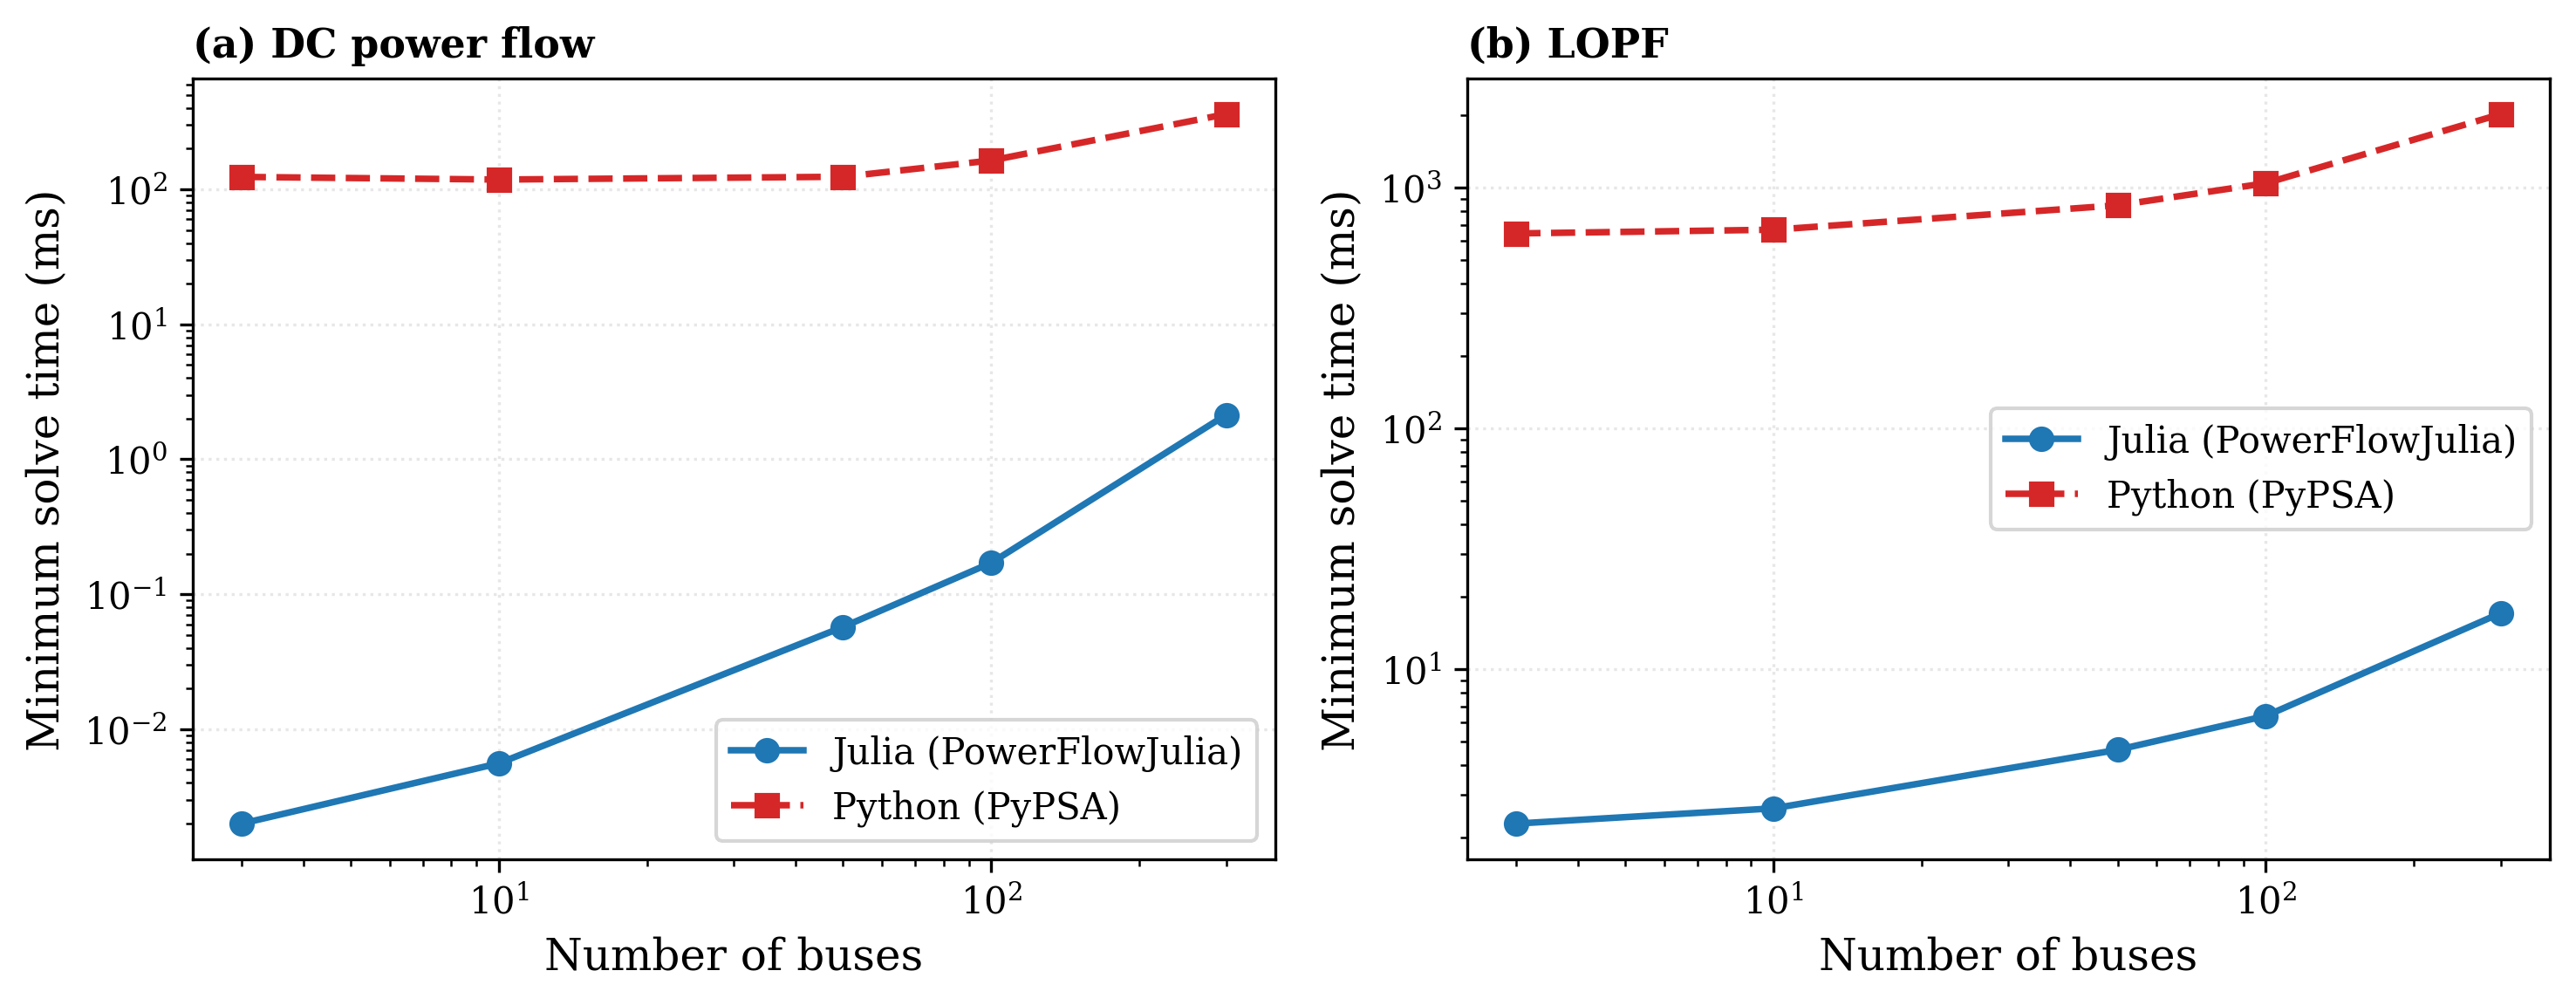
\includegraphics[width=\textwidth]{plots/fig_scaling_dcpf_lopf.png}
    \caption{Execution-time scaling of (a)~DC power flow and (b)~LOPF on synthetic networks, Julia versus PyPSA, on log--log axes. Each point is the minimum solve time over repeated samples with threads pinned.}
    \label{fig:scaling_dcpf_lopf}
\end{figure}

\begin{figure}[H]
    \centering
    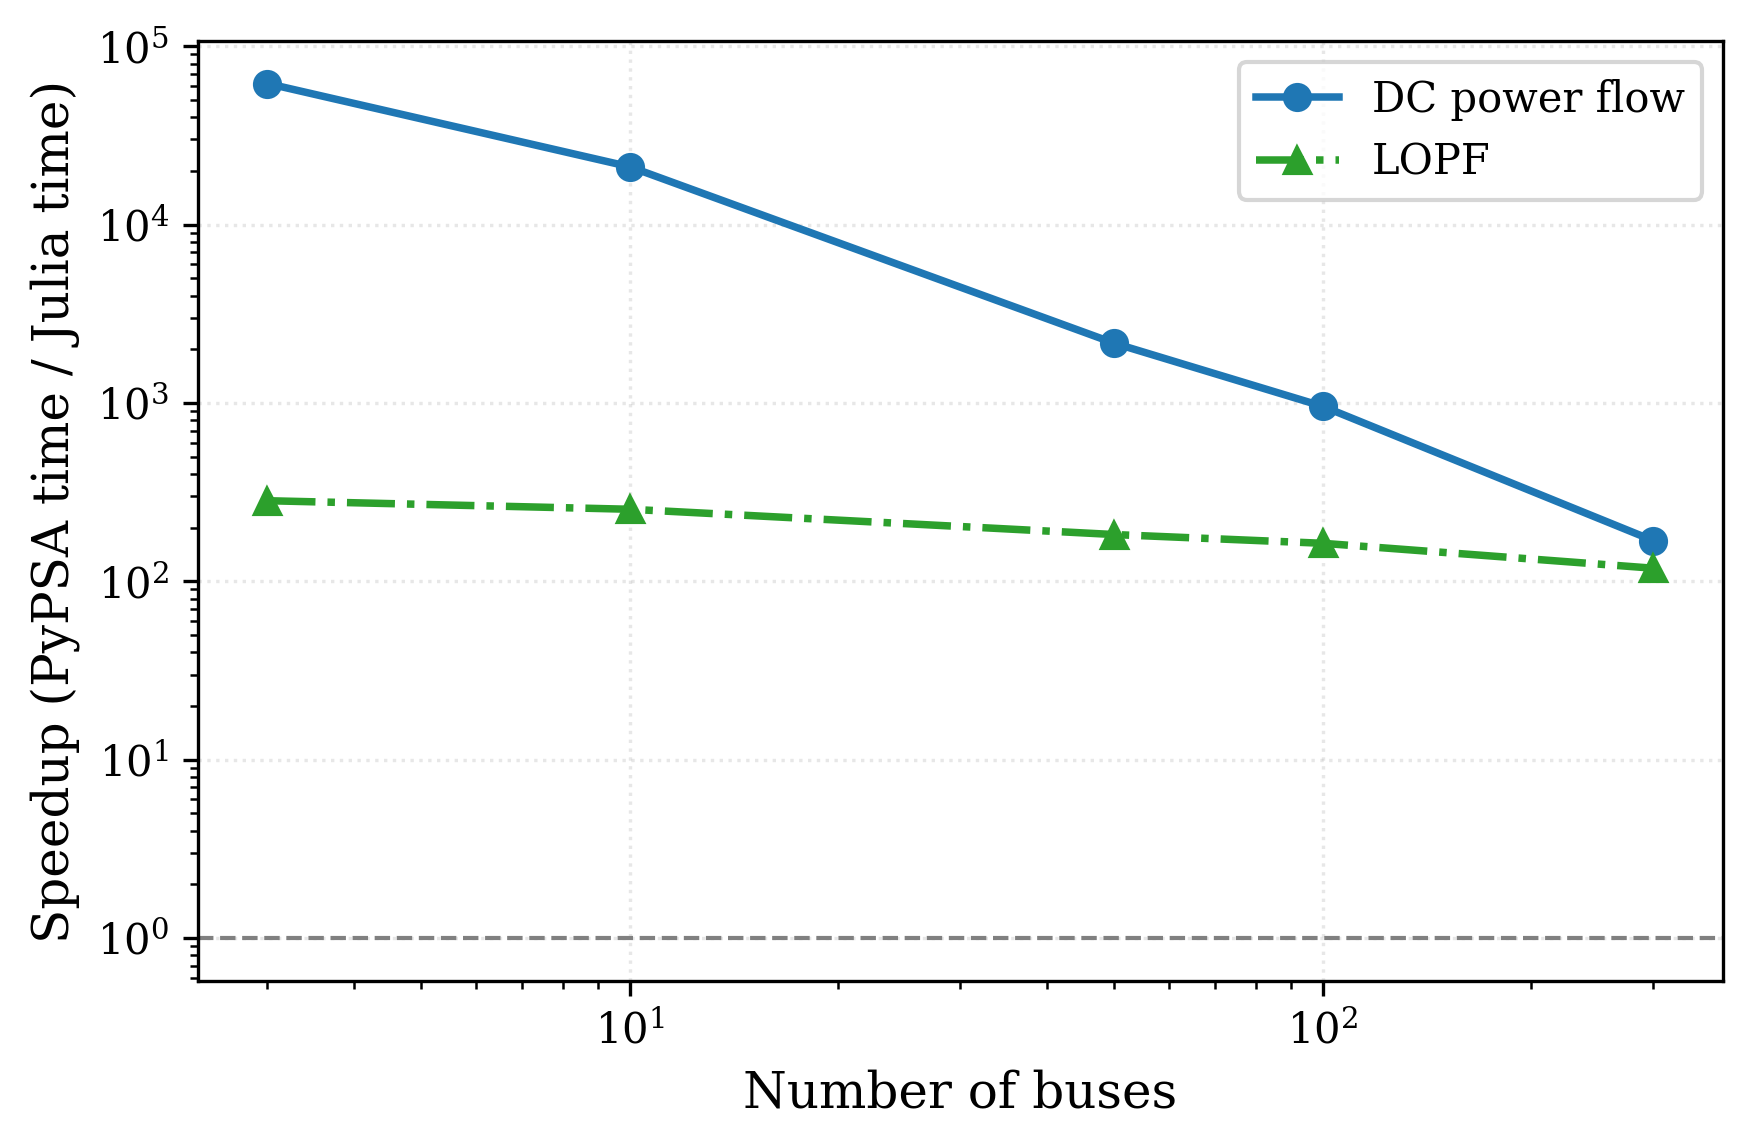
\includegraphics[width=0.7\textwidth]{plots/fig_speedup_size.png}
    \caption{Speedup of Julia over PyPSA (PyPSA time divided by Julia time) versus network size, for DC power flow and LOPF. The dashed line marks parity.}
    \label{fig:speedup_size}
\end{figure}

\begin{figure}[H]
    \centering
    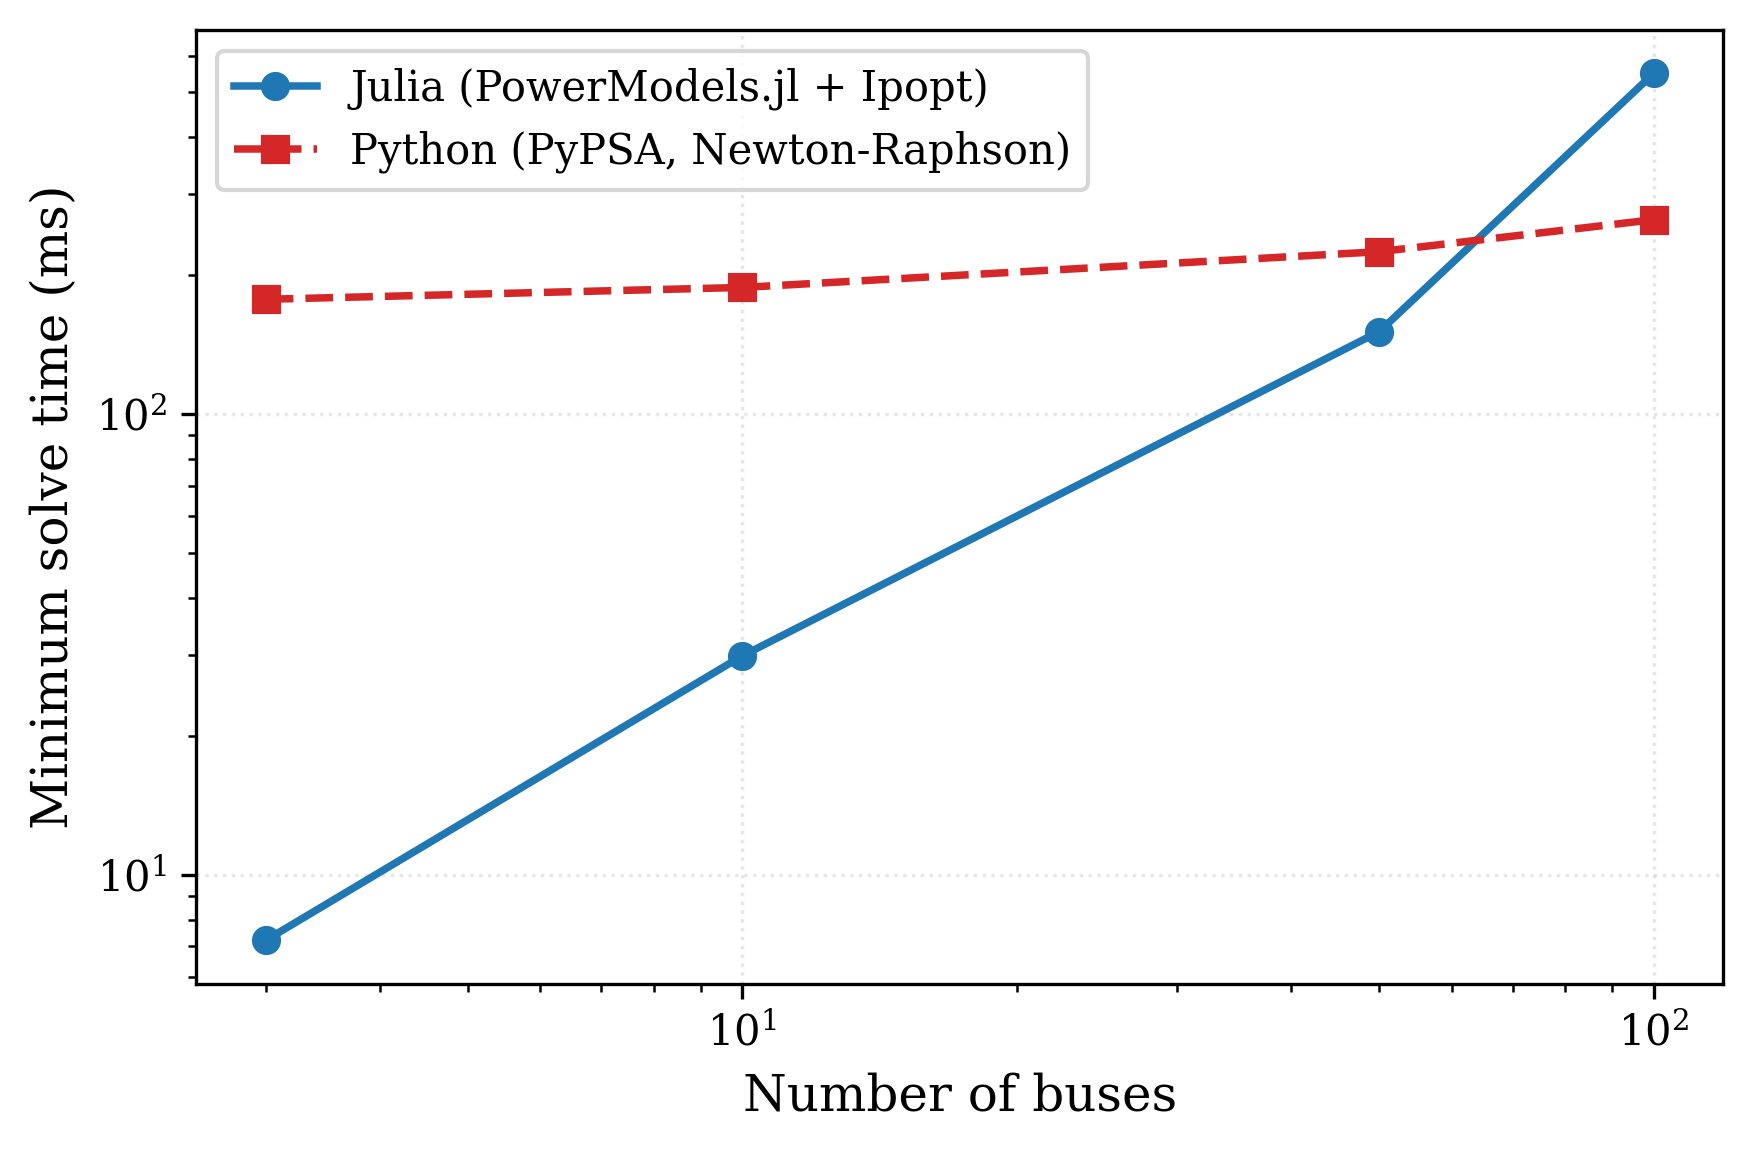
\includegraphics[width=0.7\textwidth]{plots/fig_scaling_acpf.png}
    \caption{AC power flow execution time versus network size. Julia (Ipopt) is faster only at small sizes and becomes slower than PyPSA's Newton--Raphson at 100~buses --- the one method where the porting does not yield a speedup.}
    \label{fig:scaling_acpf}
\end{figure}

\begin{figure}[H]
    \centering
    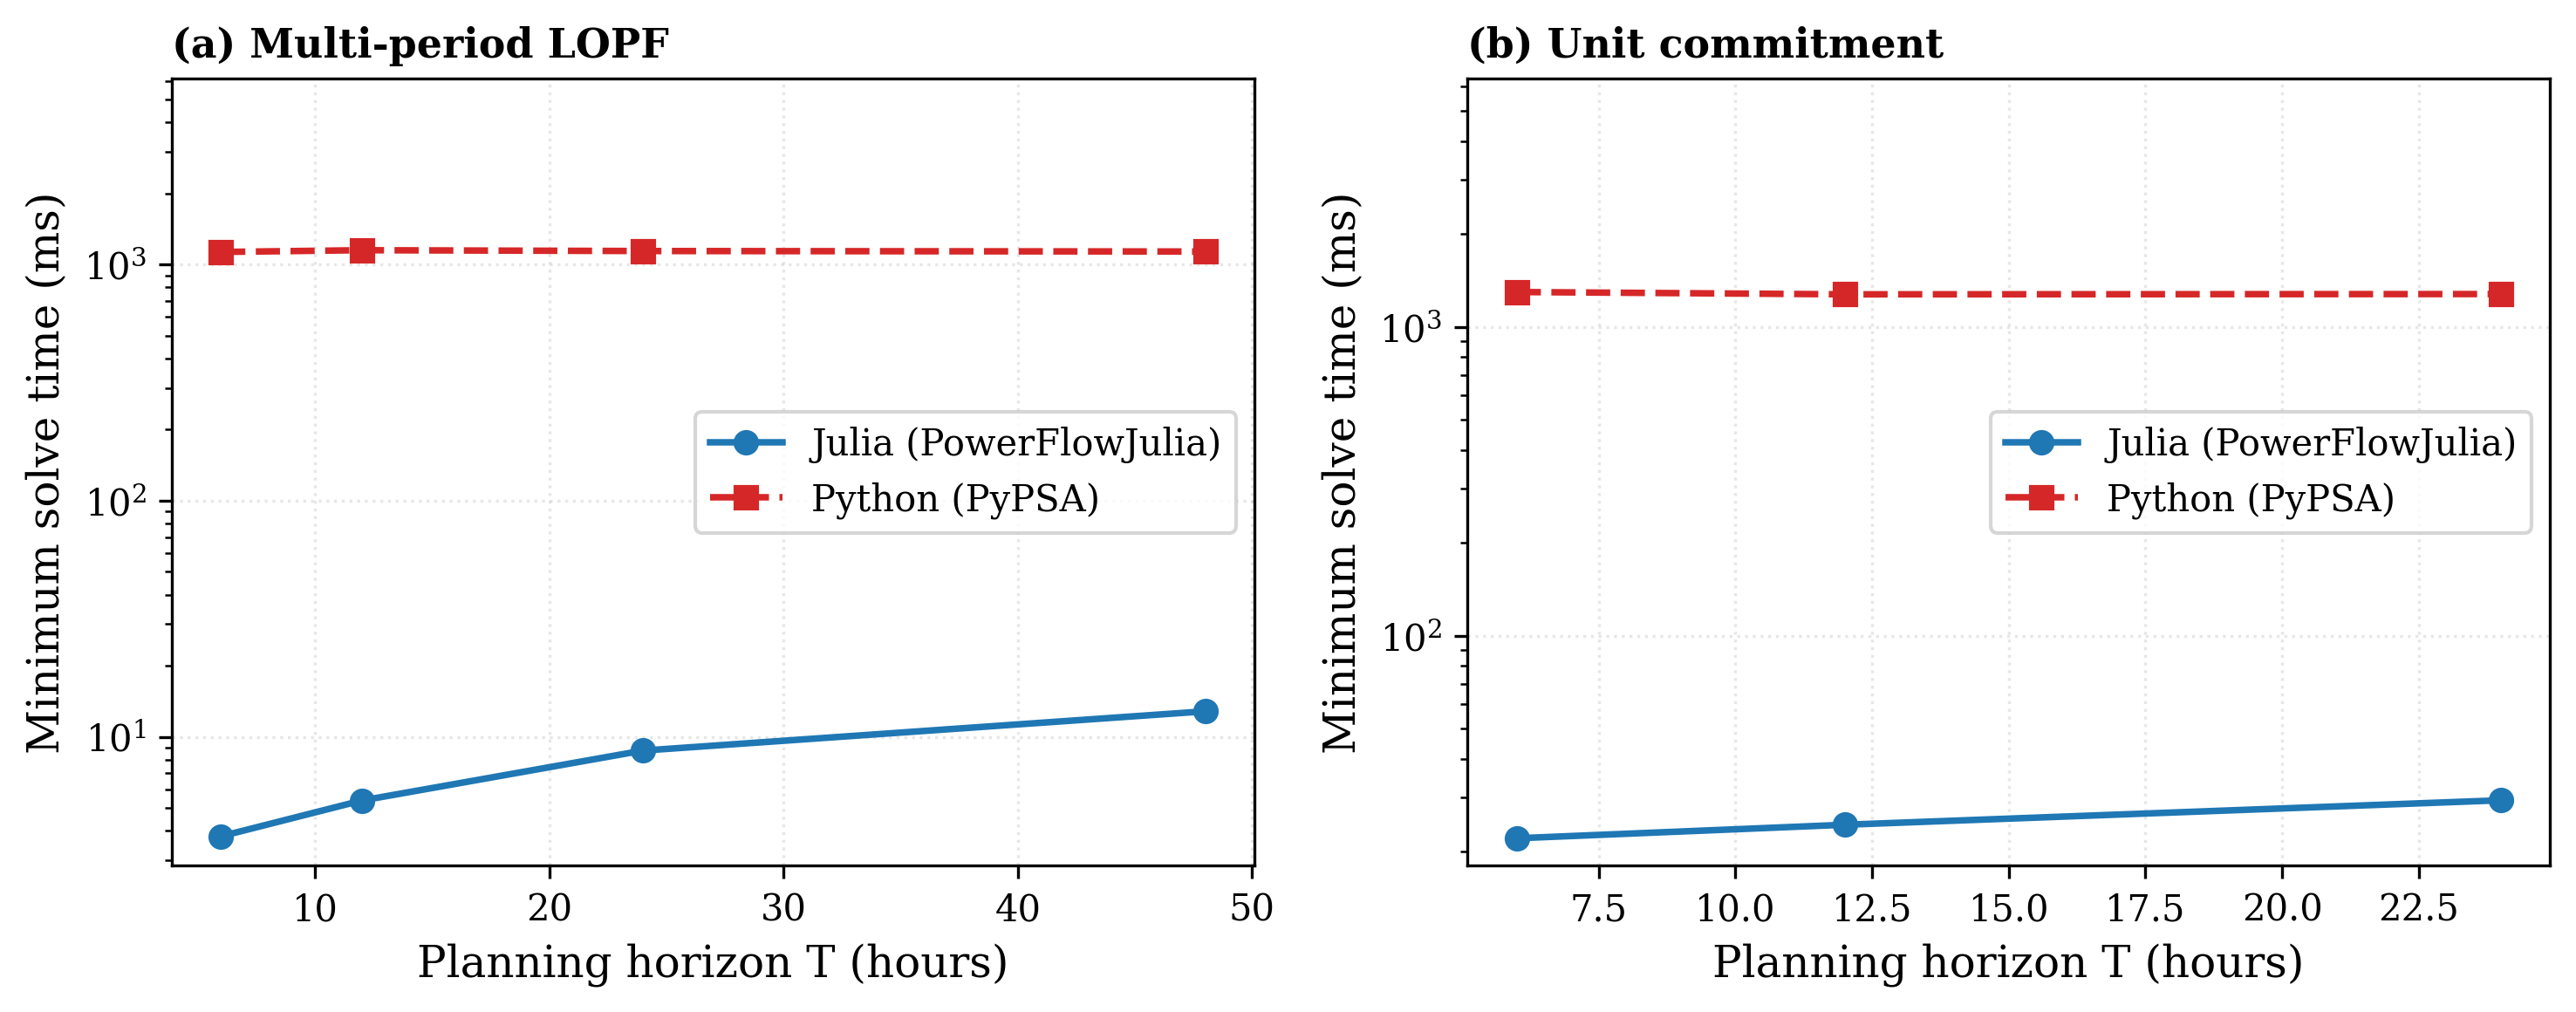
\includegraphics[width=\textwidth]{plots/fig_scaling_mp_uc.png}
    \caption{Execution time versus planning horizon for (a)~multi-period LOPF and (b)~unit commitment. PyPSA's time is nearly constant, confirming that the bottleneck is model assembly rather than solving.}
    \label{fig:scaling_mp_uc}
\end{figure}

\begin{figure}[H]
    \centering
    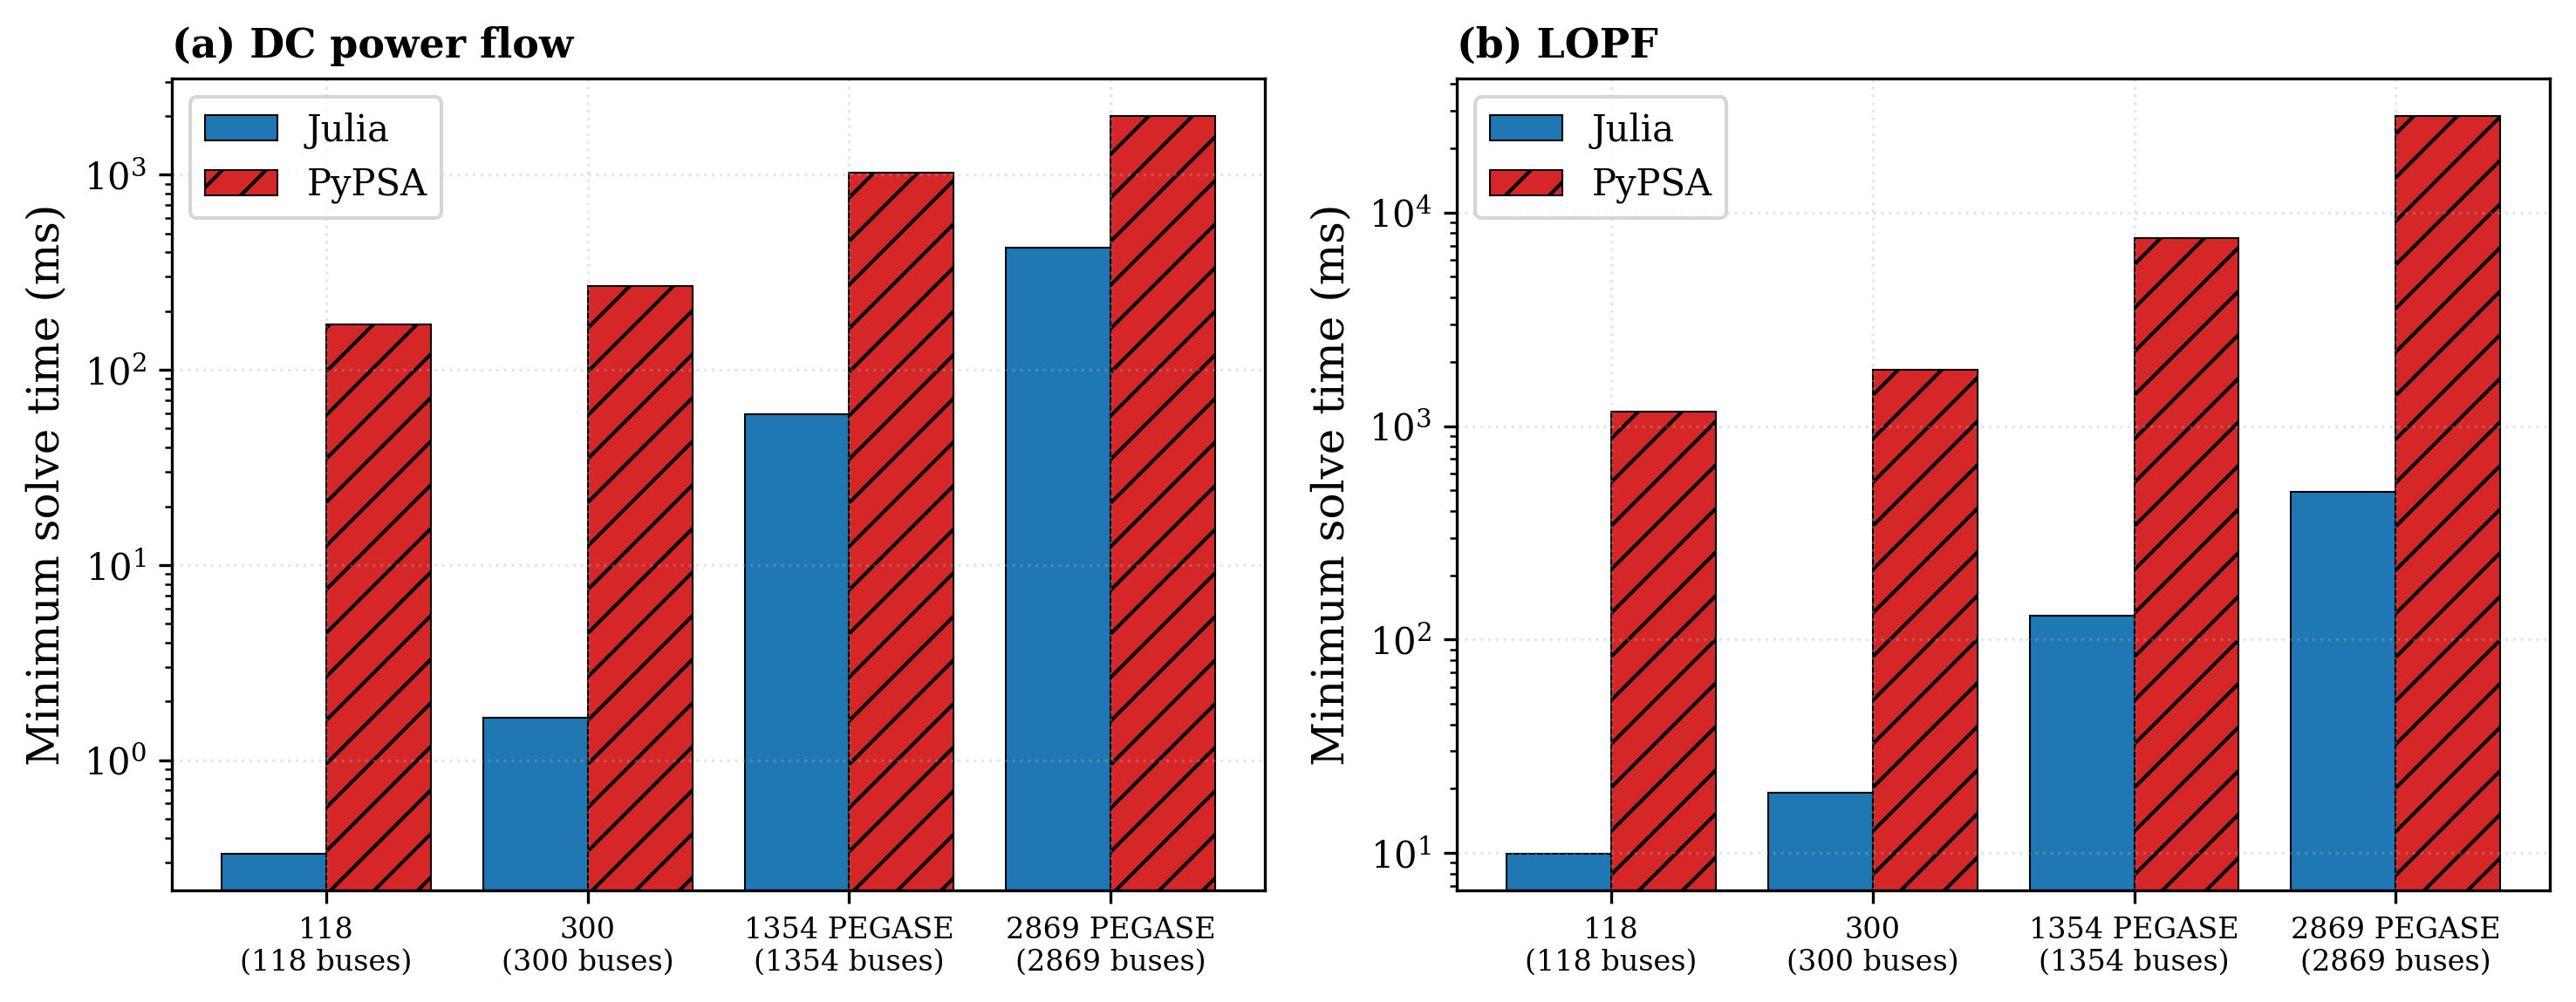
\includegraphics[width=\textwidth]{plots/fig_realcases.png}
    \caption{Minimum solve time on standard IEEE and PEGASE networks for (a)~DC power flow and (b)~LOPF, Julia versus PyPSA. The PEGASE cases are part of the real European transmission grid.}
    \label{fig:realcases}
\end{figure}

% ──────────────────────────────────────────────────────────────────────────────
\section{Network Object Model and PyPSA-Compatible API}
\label{sec:network_model}
% ──────────────────────────────────────────────────────────────────────────────

The standalone solver scripts described in previous sections accept raw tuples and dictionaries as input, which is adequate for isolated benchmarks but impractical for building complete energy system models. To address this, a typed network object model was developed in \texttt{julia/src/}, providing a PyPSA-compatible API that allows the same workflow to be used in Julia and Python.

\subsection{Component Type Hierarchy}

All network components are represented as immutable Julia \texttt{struct}s, ensuring type stability and enabling compiler optimisations. Table~\ref{tab:components} lists the implemented components with their PyPSA equivalents.

\begin{table}[H]
\centering
\caption{PowerFlowJulia component types and PyPSA equivalents}
\label{tab:components}
\begin{tabular}{lll}
\toprule
\textbf{Julia Type} & \textbf{PyPSA Equivalent} & \textbf{Key Fields} \\
\midrule
\texttt{Bus}              & \texttt{network.buses}             & \texttt{v\_nom}, \texttt{slack}, \texttt{bus\_type} \\
\texttt{Line}             & \texttt{network.lines}             & \texttt{r}, \texttt{x}, \texttt{b}, \texttt{s\_nom} \\
\texttt{Transformer}      & \texttt{network.transformers}      & \texttt{x}, \texttt{tap\_ratio}, \texttt{phase\_shift} \\
\texttt{Generator}        & \texttt{network.generators}       & \texttt{p\_nom}, \texttt{marginal\_cost}, \texttt{committable} \\
\texttt{Load}             & \texttt{network.loads}            & \texttt{p\_set}, \texttt{q\_set} \\
\texttt{StorageUnit}      & \texttt{network.storage\_units}   & \texttt{p\_nom}, \texttt{e\_nom}, $\eta^{ch}$, $\eta^{dis}$ \\
\texttt{Store}            & \texttt{network.stores}           & \texttt{e\_nom}, \texttt{p\_nom}, \texttt{standing\_loss} \\
\texttt{Carrier}          & \texttt{network.carriers}         & \texttt{co2\_emissions} \\
\texttt{Link}             & \texttt{network.links}            & \texttt{bus0}, \texttt{bus1}, \texttt{efficiency} \\
\texttt{GlobalConstraint} & \texttt{network.global\_constraints} & \texttt{carrier\_weightings}, \texttt{constant} \\
\bottomrule
\end{tabular}
\end{table}

\subsection{Network Container and API}

The \texttt{Network} struct aggregates all component dictionaries (\texttt{Dict\{String,~T\}}) and exposes a unified \texttt{add!} interface that mirrors PyPSA's \texttt{network.add()} method. All ten component types --- \texttt{Bus}, \texttt{Line}, \texttt{Transformer}, \texttt{Generator}, \texttt{Load}, \texttt{StorageUnit}, \texttt{Store}, \texttt{Carrier}, \texttt{Link}, and \texttt{GlobalConstraint} --- are accessible through the same entry point, using the same keyword argument names as PyPSA (e.g., \texttt{bus0}/\texttt{bus1} for branch endpoints, \texttt{p\_nom}, \texttt{marginal\_cost}, \texttt{s\_nom}).

The high-level \texttt{pf} and \texttt{optimize} functions dispatch to the appropriate solver based on network content: if any generator has \texttt{committable=true}, \texttt{optimize} automatically selects Unit Commitment; if $T > 1$, it selects multi-period LOPF; otherwise, single-period LOPF is used. This design allows PyPSA users to migrate with minimal changes to their existing workflow.

% ──────────────────────────────────────────────────────────────────────────────
\section{Transformer Tap-Ratio Correction}
\label{sec:transformer}
% ──────────────────────────────────────────────────────────────────────────────

The IEEE 14-bus network contains four transformers with off-nominal tap ratios ($a \in \{0.932, 0.969, 0.978\}$). The standard DC power flow formulation ignores these ratios, treating transformers as ordinary lines. This introduces systematic angle errors at buses downstream of transformers.

\subsection{Corrected Transformer Model}

Following the PyPSA and MATPOWER simplified DC convention, the effective susceptance of a transformer with off-nominal tap ratio $a$ and reactance $x$ is:

\begin{equation}
    b_\text{eff} = \frac{S_\text{base}}{x \cdot a}.
    \label{eq:tap_correction}
\end{equation}

For phase-shifting transformers with shift angle $\varphi$ (degrees), the power balance right-hand side is modified by an equivalent injection:

\begin{equation}
    P_\text{shift}[k] += b_\text{eff} \cdot \varphi_\text{rad}, \qquad
    P_\text{shift}[m] -= b_\text{eff} \cdot \varphi_\text{rad},
    \label{eq:phase_shift}
\end{equation}

and the branch flow becomes $P_{km} = b_\text{eff}(\theta_k - \theta_m - \varphi_\text{rad})$.

\subsection{Validation on IEEE 14-Bus}

Table~\ref{tab:tap_correction} compares DC power flow accuracy on the IEEE 14-bus network with and without tap-ratio correction, measured against the MATPOWER full-AC reference.

\begin{table}[H]
\centering
\caption{DC power flow accuracy on IEEE 14-bus: tap-corrected vs.\ tap-ignored}
\label{tab:tap_correction}
\begin{tabular}{lrrr}
\toprule
\textbf{Metric} & \textbf{With tap correction} & \textbf{Without correction} & \textbf{Improvement} \\
\midrule
Max $|\Delta\theta|$ (deg) & 1.15 & 1.39 & 17.3\% \\
MAE (deg)                  & 0.57 & 0.73 & 21.2\% \\
\bottomrule
\end{tabular}
\end{table}

The tap-ratio correction reduces the mean absolute angle error by 21.2\%, with the largest improvements at buses 6, 9--14, which are electrically downstream of the corrected transformers. The residual error ($0.57^\circ$) is an inherent limitation of the lossless DC approximation, not a software defect.

% ──────────────────────────────────────────────────────────────────────────────
\section{Locational Marginal Prices}
\label{sec:lmp}
% ──────────────────────────────────────────────────────────────────────────────

Locational Marginal Prices (LMPs) represent the marginal cost of supplying one additional megawatt of load at a given bus~\cite{schweppe1988}. In the DC LOPF, they are the dual variables (shadow prices) of the nodal power balance constraints:

\begin{equation}
    \lambda_k = -\frac{\partial \text{obj}^*}{\partial P_k^\text{load}},
    \label{eq:lmp_def}
\end{equation}

where $\text{obj}^*$ is the optimal generation cost and $P_k^\text{load}$ is the load at bus $k$.

\subsection{Implementation}

LMPs are extracted directly from the JuMP model after the LOPF solve. The balance constraint at each bus $k$ is stored with a reference label, and the dual is retrieved post-solution:

\begin{lstlisting}[language=Julia, caption={LMP extraction from JuMP dual variables}, label={lst:lmp}]
# Store labelled balance constraints
balance_con = Vector{Any}(undef, n)
for k in 1:n
    balance_con[k] = @constraint(model,
        sum(B[k,m]*theta[m] for m in 1:n) == gen_inj - P_load[k] + P_shift[k])
end
optimize!(model)
# LMP = -dual(balance_con[k])
# Sign: load appears as -P_load on RHS, so d(obj)/d(P_load) = -dual
lmp = Dict(bus_names[k] => -dual(balance_con[k]) for k in 1:n)
\end{lstlisting}

\subsection{Validation}

Three scenarios verify the correctness of the LMP implementation:

\begin{enumerate}
    \item \textbf{Uncongested single-bus}: one generator at $c = 20\,\text{\euro/MWh}$ produces $\lambda = 20\,\text{\euro/MWh}$ --- the LMP equals the marginal cost.
    \item \textbf{Uncongested 3-bus}: all LMPs are equal to the marginal generator cost ($50\,\text{\euro/MWh}$ when G2 is the marginal unit), confirming no spatial price differentiation without congestion.
    \item \textbf{Congested 2-bus}: a 80\,MW line limit between a cheap area ($c_1 = 10\,\text{\euro/MWh}$) and an expensive area ($c_2 = 60\,\text{\euro/MWh}$) produces $\lambda_1 = 10$ and $\lambda_2 = 60\,\text{\euro/MWh}$, with a \emph{congestion rent} of $50\,\text{\euro/MWh}$ --- the classical result from electricity market theory.
\end{enumerate}

For the multi-period LOPF, time-varying LMPs $\lambda_k(t)$ are extracted from the per-period balance constraints, enabling analysis of how nodal prices evolve with load and renewable generation profiles.

% ──────────────────────────────────────────────────────────────────────────────
\section{Unit Commitment}
\label{sec:uc}
% ──────────────────────────────────────────────────────────────────────────────

Unit Commitment (UC) extends the LOPF by adding binary on/off decisions for generators, minimum operating constraints, and startup/shutdown costs. It is formulated as a Mixed-Integer Linear Program (MILP).

\subsection{Mathematical Formulation}

For each committable generator $g$ and time period $t$, three binary variables are introduced: $u_{g,t} \in \{0,1\}$ (commitment status), $\sigma_{g,t}^+$ (startup), and $\sigma_{g,t}^-$ (shutdown). The extended objective and key constraints are:

\begin{align}
    \min \quad & \sum_{g,t} \left[ c_g P_{g,t} + C_g^{su}\,\sigma_{g,t}^+ + C_g^{sd}\,\sigma_{g,t}^- \right]
    \label{eq:uc_obj} \\
    \text{s.t.} \quad
    & u_{g,t} - u_{g,t-1} = \sigma_{g,t}^+ - \sigma_{g,t}^-
    \label{eq:uc_transition} \\
    & p_g^\text{min} u_{g,t} \leq P_{g,t} \leq p_g^\text{max} u_{g,t}
    \label{eq:uc_dispatch} \\
    & \sum_{\tau = t - T_g^{up}+1}^{t} \sigma_{g,\tau}^+ \leq u_{g,t},
    \quad \forall t \geq T_g^{up}
    \label{eq:uc_minup} \\
    & \sum_{\tau = t - T_g^{dn}+1}^{t} \sigma_{g,\tau}^- \leq 1 - u_{g,t},
    \quad \forall t \geq T_g^{dn}
    \label{eq:uc_mindn}
\end{align}

where $C_g^{su}$, $C_g^{sd}$ are startup/shutdown costs [\euro], and $T_g^{up}$, $T_g^{dn}$ are minimum up/down times [hours].

\subsection{Implementation}

The UC solver is implemented in \texttt{julia/src/unit\_commitment.jl} and uses HiGHS as the MILP solver via JuMP. After the MILP solve, binary variables are fixed at their optimal values and a LP relaxation is re-solved to extract price-consistent LMPs --- the standard approach in electricity markets~\cite{oneill2005}. A generator is identified as committable by setting \texttt{committable=true} in the \texttt{Generator} struct, together with UC-specific fields (\texttt{min\_up\_time}, \texttt{min\_down\_time}, \texttt{startup\_cost}, \texttt{shutdown\_cost}, \texttt{initial\_status}) that map directly to the parameters of Equations~\eqref{eq:uc_logic}--\eqref{eq:uc_obj_ch2}.

\subsection{Validation}

Table~\ref{tab:uc_result} shows the 24-hour commitment schedule for a 3-bus network with a baseload unit (cheap, slow-start) and a peaker (expensive, fast-start).

\begin{table}[H]
\centering
\caption{Unit Commitment: 24-hour commitment schedule (1=ON, 0=OFF)}
\label{tab:uc_result}
\begin{tabular}{lcc}
\toprule
\textbf{Generator} & \textbf{Hours ON} & \textbf{Total starts} \\
\midrule
BaseLoad (15\,\euro/MWh, $T^{up}=4$\,h) & 9--21 (13\,h) & 1 \\
Peaker   (70\,\euro/MWh, $T^{up}=1$\,h) & 1--24 (24\,h) & 1 \\
\bottomrule
\end{tabular}
\end{table}

The MILP correctly schedules the cheap baseload unit during high-demand hours (9--21) while the more expensive peaker covers the residual. The minimum up-time constraint ($T_g^{up} = 4$\,h) is respected: once baseload starts, it operates for at least 4 consecutive hours. The average LMP across all buses is 40.2\,\euro/MWh, reflecting the weighted mix of baseload and peaker marginal costs over the 24-hour horizon.

\subsection{Unit Commitment Performance}

Table~\ref{tab:uc_benchmark_t} reports UC solve times as a function of planning horizon $T$, and Table~\ref{tab:uc_benchmark_scale} reports scaling with network size at fixed $T = 24$.

\begin{table}[H]
\centering
\caption{Unit Commitment benchmark: Julia (JuMP+HiGHS) vs PyPSA (linopy+HiGHS), 3-bus network, varying horizon, minimum time}
\label{tab:uc_benchmark_t}
\begin{tabular}{rrrr}
\toprule
\textbf{T (hours)} & \textbf{Julia (ms)} & \textbf{PyPSA (ms)} & \textbf{Speedup} \\
\midrule
  6 &  22.11 & 1{,}298 &  59$\times$ \\
 12 &  24.45 & 1{,}276 &  52$\times$ \\
 24 &  29.35 & 1{,}278 &  44$\times$ \\
\bottomrule
\end{tabular}
\end{table}

\begin{table}[H]
\centering
\caption{Unit Commitment benchmark: Julia vs PyPSA, $T=24$\,h, varying network size, minimum time}
\label{tab:uc_benchmark_scale}
\begin{tabular}{rrrr}
\toprule
\textbf{Buses} & \textbf{Julia (ms)} & \textbf{PyPSA (ms)} & \textbf{Speedup} \\
\midrule
  3 &   8.49 &   671 & 79$\times$ \\
 14 &  42.56 &   730 & 17$\times$ \\
 30 &  63.20 & 1{,}510 & 24$\times$ \\
\bottomrule
\end{tabular}
\end{table}

The UC speedup ($17$--$79\times$) is lower than for the continuous LOPF because the dominant time shifts from model construction toward MILP branch-and-bound search, which both implementations delegate to the same HiGHS solver. The PyPSA solve time is again dominated by a large fixed model-assembly overhead. The scaling with network size is non-monotonic, reflecting the combinatorial variability of the branch-and-bound search across the (synthetic) instances rather than a smooth trend.


% ──────────────────────────────────────────────────────────────────────────────
\section{AI Component: LSTM Load Forecasting and Stochastic Dispatch}
\label{sec:ai_component}
% ──────────────────────────────────────────────────────────────────────────────

The preceding sections addressed solver performance. This section introduces the AI component that justifies the "AI-assisted" framing of the thesis: an LSTM-based load forecaster with conformal prediction intervals, whose output drives a scenario-based stochastic LOPF. The implementation is contained in \texttt{julia/src/forecasting.jl} and \texttt{julia/src/stochastic\_lopf.jl}.

\subsection{Training Data}

The forecaster is trained and evaluated on \textbf{real} hourly load data for Germany, published by Open Power System Data (OPSD) from the ENTSO-E Transparency Platform \cite{opsd2020timeseries}. The cleaned series (\texttt{data/opsd\_de\_load.csv}) covers 1{,}155 complete days (2017-08-03 to 2020-09-30; peak $77{,}549$\,MW, mean $55{,}593$\,MW), peak-normalized to per-unit. A population-weighted hourly temperature series (\texttt{data/opsd\_de\_temp.csv}, six German cities, ERA5 reanalysis) is available as an optional exogenous feature. Evaluation uses a strict \emph{out-of-time} split: the LSTM is trained on the earliest 1{,}095 days and tested on the final 60 days, which it never sees during training. Because neural-network initialization is stochastic, every figure is reported as the mean $\pm$ standard deviation over three random seeds. A synthetic generator (\texttt{generate\_synthetic\_data}) is retained only as a reproducible fallback for the demonstration pipeline and unit tests.

\subsection{Forecast Quality on Real Data}
\label{sec:forecast_quality}

The honest test of a learned forecaster is whether it beats the trivial baselines on data it has never seen. Table~\ref{tab:forecast_metrics} reports the out-of-time accuracy of the LSTM against the persistence baseline (tomorrow $=$ today) and the seasonal-naive baseline (each hour $=$ the same hour one week earlier), both with and without the temperature feature.

\begin{table}[H]
\centering
\caption{Out-of-time forecast accuracy on real German load (60-day test, mean $\pm$ std over 3 seeds). Lower is better}
\label{tab:forecast_metrics}
\begin{tabular}{lccc}
\toprule
\textbf{Method} & \textbf{MAPE (\%)} & \textbf{RMSE (pu)} & \textbf{RMSE skill vs seasonal} \\
\midrule
Seasonal-naive             & \textbf{2.77} & \textbf{0.0243} & --- \\
LSTM $+$ temperature$^{*}$ & $3.67 \pm 0.68$ & $0.0300$ & $-23.4\%$ \\
LSTM (calendar only)       & $5.83 \pm 0.53$ & $0.0447$ & $-83.6\%$ \\
Persistence                & 7.73 & 0.0780 & --- \\
\bottomrule
\end{tabular}
\end{table}

\noindent$^{*}$ The temperature feature uses the \emph{actual} target-day temperature as a perfect-forecast proxy; this is an idealization, stated honestly, that upper-bounds the achievable gain from weather information.

The result is reported as it is, without spin. The LSTM \textbf{beats persistence} comfortably ($+42.7\%$ RMSE skill without temperature, $+61.5\%$ with it), but it \textbf{does not beat the seasonal-naive baseline}: with calendar features alone it is almost twice as inaccurate ($5.83\%$ versus $2.77\%$ MAPE), and even with idealized temperature it remains $23\%$ behind on average, although the best seed reaches parity ($+0.6\%$). This is a known property of aggregate national load: the weekly cycle that seasonal-naive copies for free is nearly deterministic, and a learned model adds value only through an exogenous signal --- here, weather, which is confirmed to be the decisive lever (it closes the gap from $-84\%$ to $-23\%$). The honest conclusion is that the contribution of the AI component is \emph{not} point-forecast accuracy but the calibrated uncertainty quantification developed in the next subsection, which the naive baselines cannot provide at all.

Figure~\ref{fig:ml_accuracy} visualizes the accuracy ranking; the strong seasonal-naive baseline (dashed line) sits below the LSTM in both configurations.

\begin{figure}[H]
    \centering
    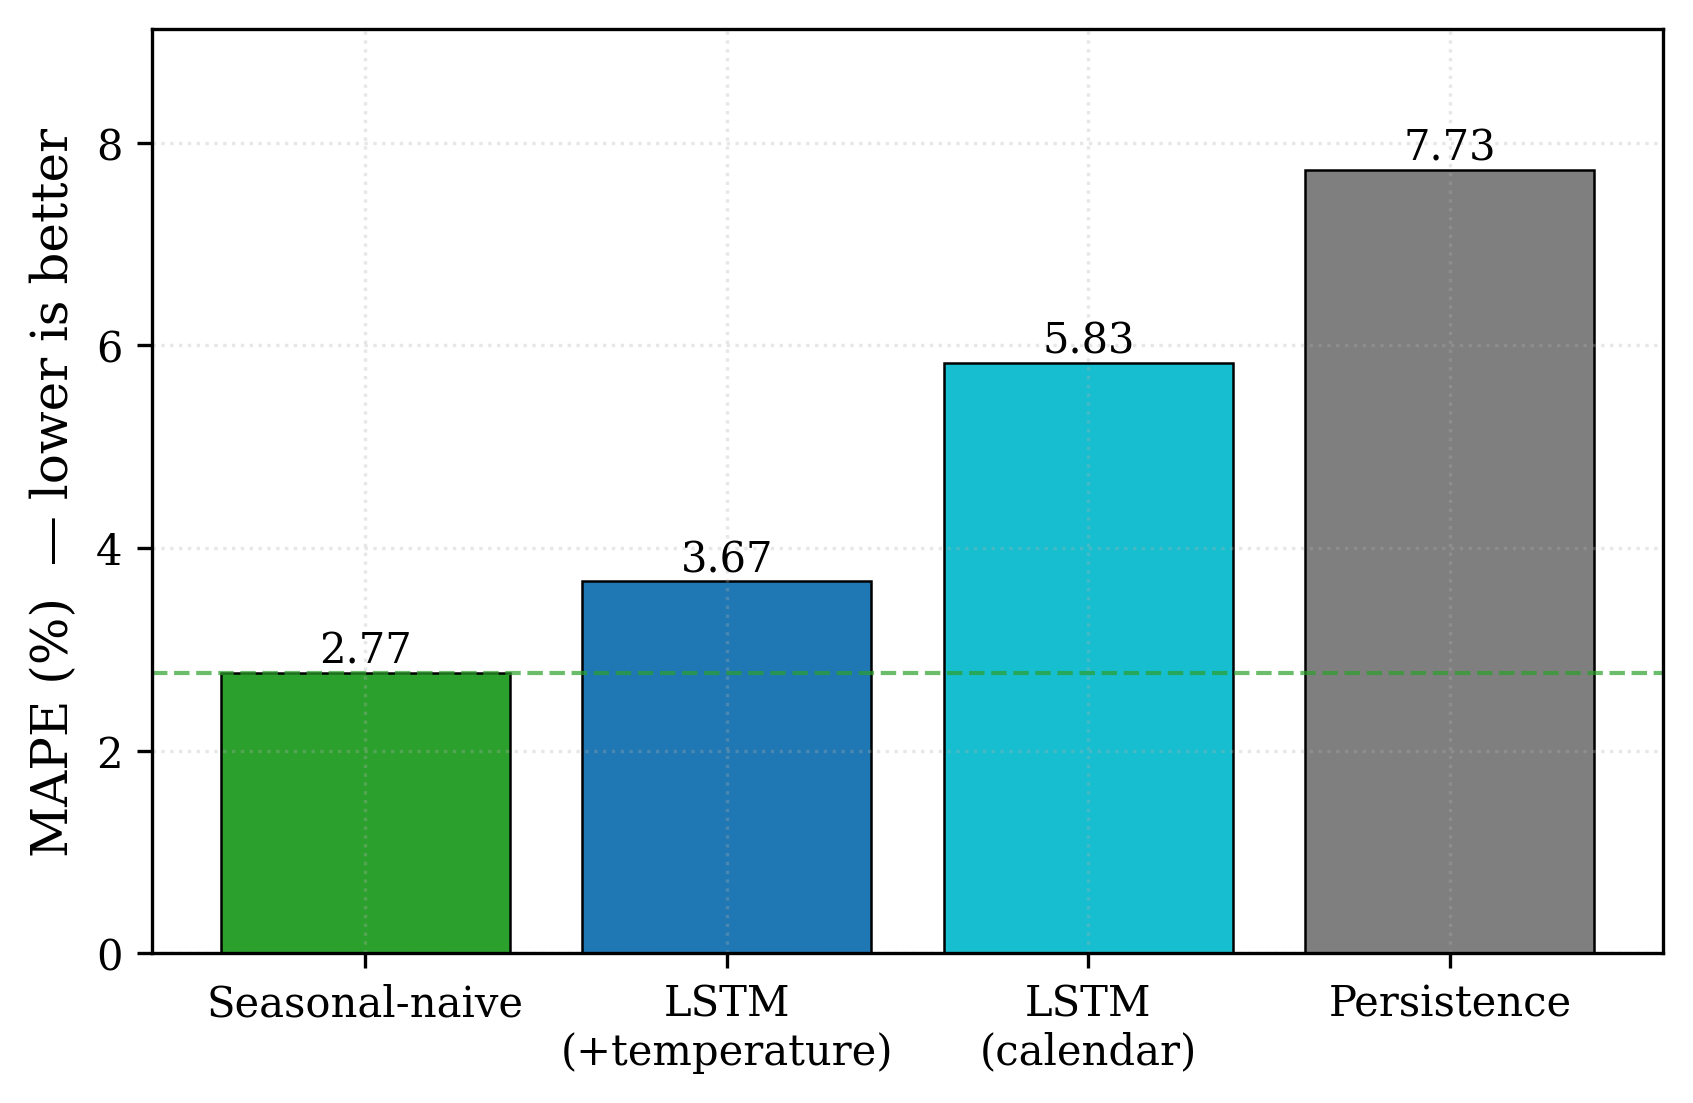
\includegraphics[width=0.7\textwidth]{plots/fig_ml_accuracy.png}
    \caption{Out-of-time forecast accuracy (MAPE) on real German load. The seasonal-naive baseline is the most accurate; the LSTM beats only persistence, and temperature narrows but does not close the gap.}
    \label{fig:ml_accuracy}
\end{figure}

Although the LSTM is not the most accurate point forecaster, it provides what the naive baselines cannot: a calibrated prediction interval. Figure~\ref{fig:ml_forecast} shows one out-of-time day with the LSTM forecast, the actual load, and the 90\% conformal band. Over the full 60-day test block the empirical coverage of the band is $100\%$, comfortably above the nominal $90\%$ guarantee --- the interval is conservative because the non-conformity score is the per-day maximum absolute error, which sizes a uniform band to the worst hour.

\begin{figure}[H]
    \centering
    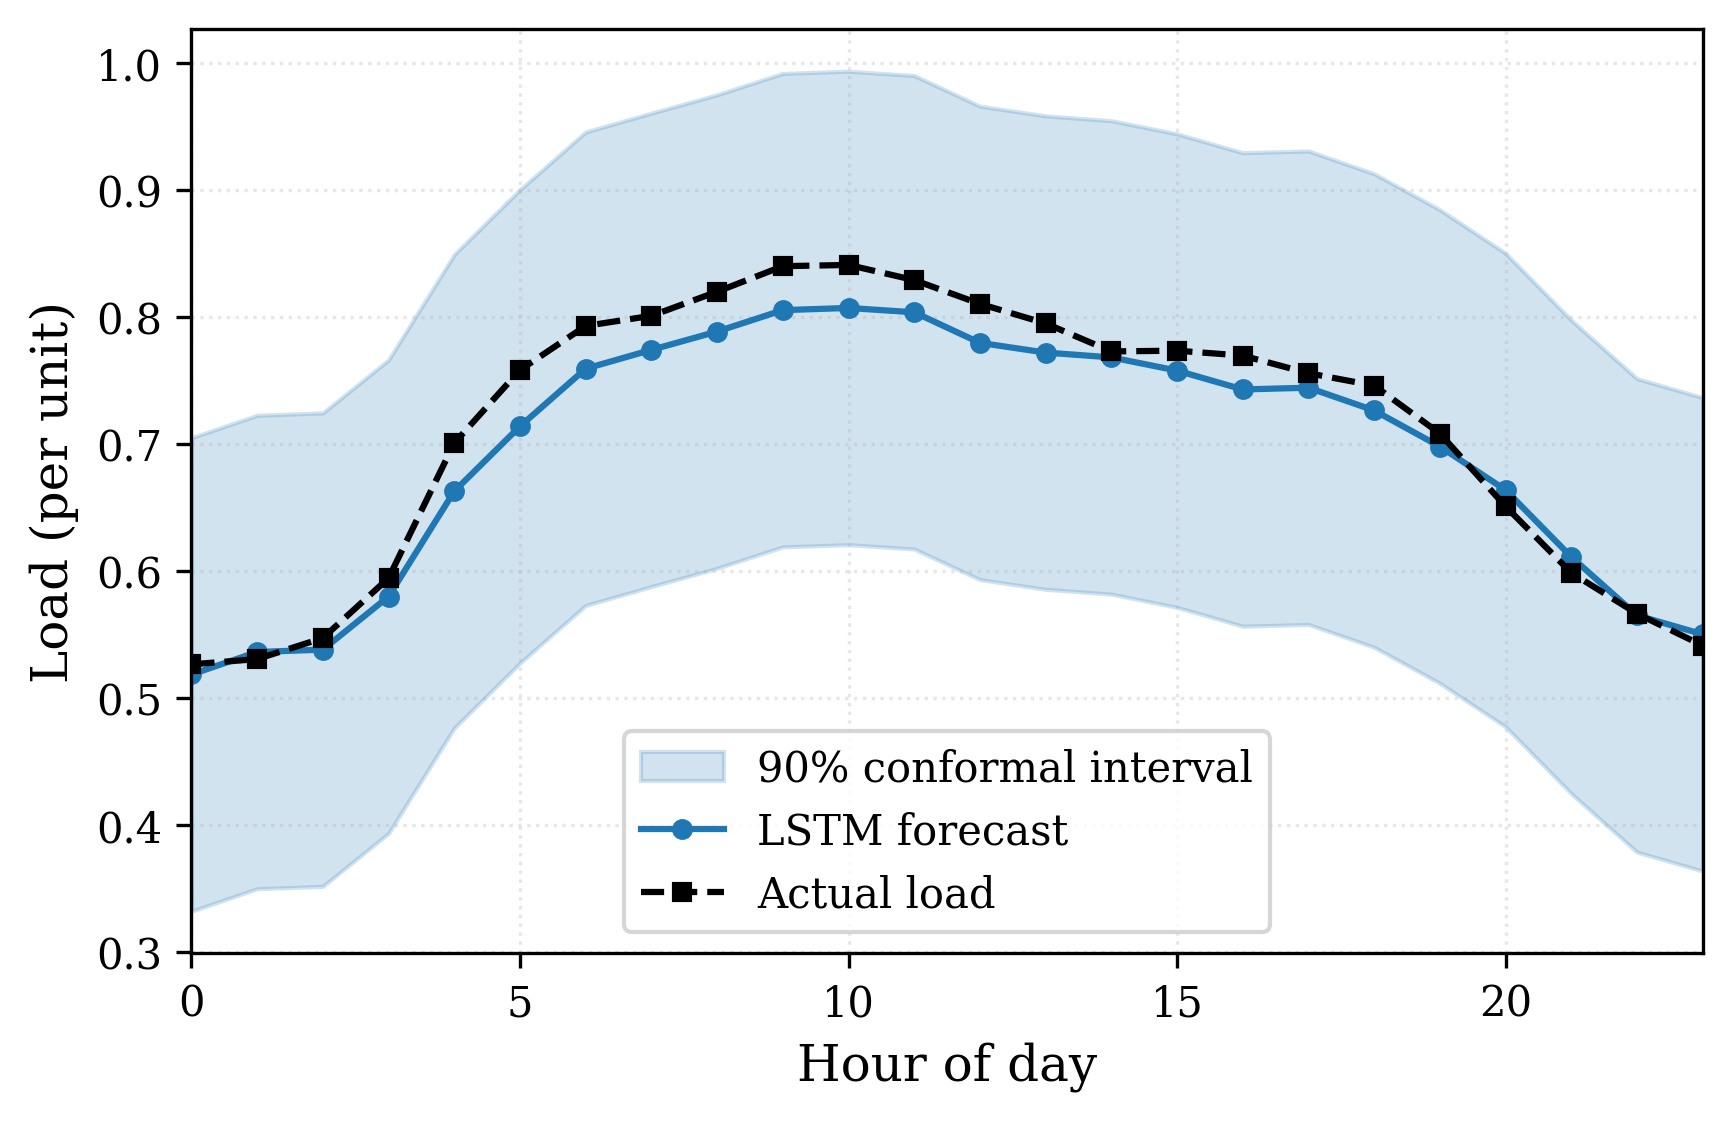
\includegraphics[width=0.7\textwidth]{plots/fig_ml_forecast.png}
    \caption{LSTM day-ahead forecast (weather-informed) with its 90\% conformal prediction interval, against the actual load, on an out-of-time test day. The forecast tracks the observed shape and the actual load stays within the band.}
    \label{fig:ml_forecast}
\end{figure}

\subsection{Stochastic LOPF: Propagating Forecast Uncertainty}

This subsection demonstrates the substantive contribution of the AI component: turning the calibrated forecast intervals into a risk-aware dispatch. The mechanism is illustrated on the 3-bus test network (Section~\ref{sec:test_network_definition}) with $T = 24$ hours, which keeps the optimization small enough to expose the cost distribution clearly. Three dispatch strategies are compared:

\begin{enumerate}
    \item \textbf{Static profile:} deterministic LOPF with a fixed default load profile (\texttt{DEFAULT\_LOAD\_PROFILE}) --- the simplest non-forecast baseline.
    \item \textbf{Point forecast:} deterministic LOPF with the forecaster's mean profile.
    \item \textbf{Stochastic SAA:} seven load scenarios sampled from the conformal intervals; an independent LOPF is solved per scenario and the costs are aggregated by Sample Average Approximation.
\end{enumerate}

Table~\ref{tab:stochastic_results} summarises the cost outcomes; the figures are illustrative of the mechanism on this demonstration network rather than a system-level economic claim.

\begin{table}[H]
\centering
\caption{Dispatch cost comparison: static profile vs point forecast vs stochastic LOPF on the sample out-of-time day ($T=24$\,h)}
\label{tab:stochastic_results}
\begin{tabular}{lrr}
\toprule
\textbf{Strategy} & \textbf{Total cost (\euro)} & \textbf{vs static} \\
\midrule
Static profile                    & 320{,}328 & --- \\
Point forecast (deterministic)    & 233{,}157 & $-27.2\%$ \\
Stochastic SAA --- $\mathbb{E}[\text{cost}]$ & 236{,}080 & $-26.3\%$ \\
Stochastic SAA --- CVaR$_{90}$              & 261{,}283 & $-18.4\%$ \\
Stochastic SAA --- best scenario            & 214{,}145 & $-33.1\%$ \\
Stochastic SAA --- worst scenario           & 264{,}649 & $-17.4\%$ \\
Stochastic SAA --- std dev                  & 13{,}895 & --- \\
\bottomrule
\end{tabular}
\end{table}

The point to take from Table~\ref{tab:stochastic_results} is \emph{not} the headline cost difference --- using the shaped forecast instead of a flat static profile naturally lowers cost on this day ($-27.2\%$), but that is a comparison against a deliberately weak baseline on a small demonstration network, so it is not advanced as a system-level result. The substantive output is the \textbf{risk profile} that only the stochastic formulation produces. Sampling demand scenarios across the calibrated conformal band and solving each yields an expected cost of $236{,}080$\,\euro, a worst-case (CVaR$_{90}$) of $261{,}283$\,\euro, and a spread of $\sigma = 13{,}895$\,\euro. The gap between expected and worst-case cost ($\approx 25{,}000$\,\euro, $+10.7\%$) is the reserve a risk-averse operator must budget to cover the worst $10\%$ of demand outcomes. \textbf{This risk quantification is the contribution of the AI layer, and it is inaccessible to any deterministic dispatch} --- including one driven by the more accurate seasonal-naive forecast, which returns a single number with no notion of uncertainty.

Figure~\ref{fig:scenario_costs} shows the resulting distribution of dispatch costs across the sampled scenarios, with the expected cost and the CVaR$_{90}$ marked. The spread of the distribution and the gap between the expected and worst-case cost are exactly the risk information that the stochastic formulation adds over a single deterministic solve.

\begin{figure}[H]
    \centering
    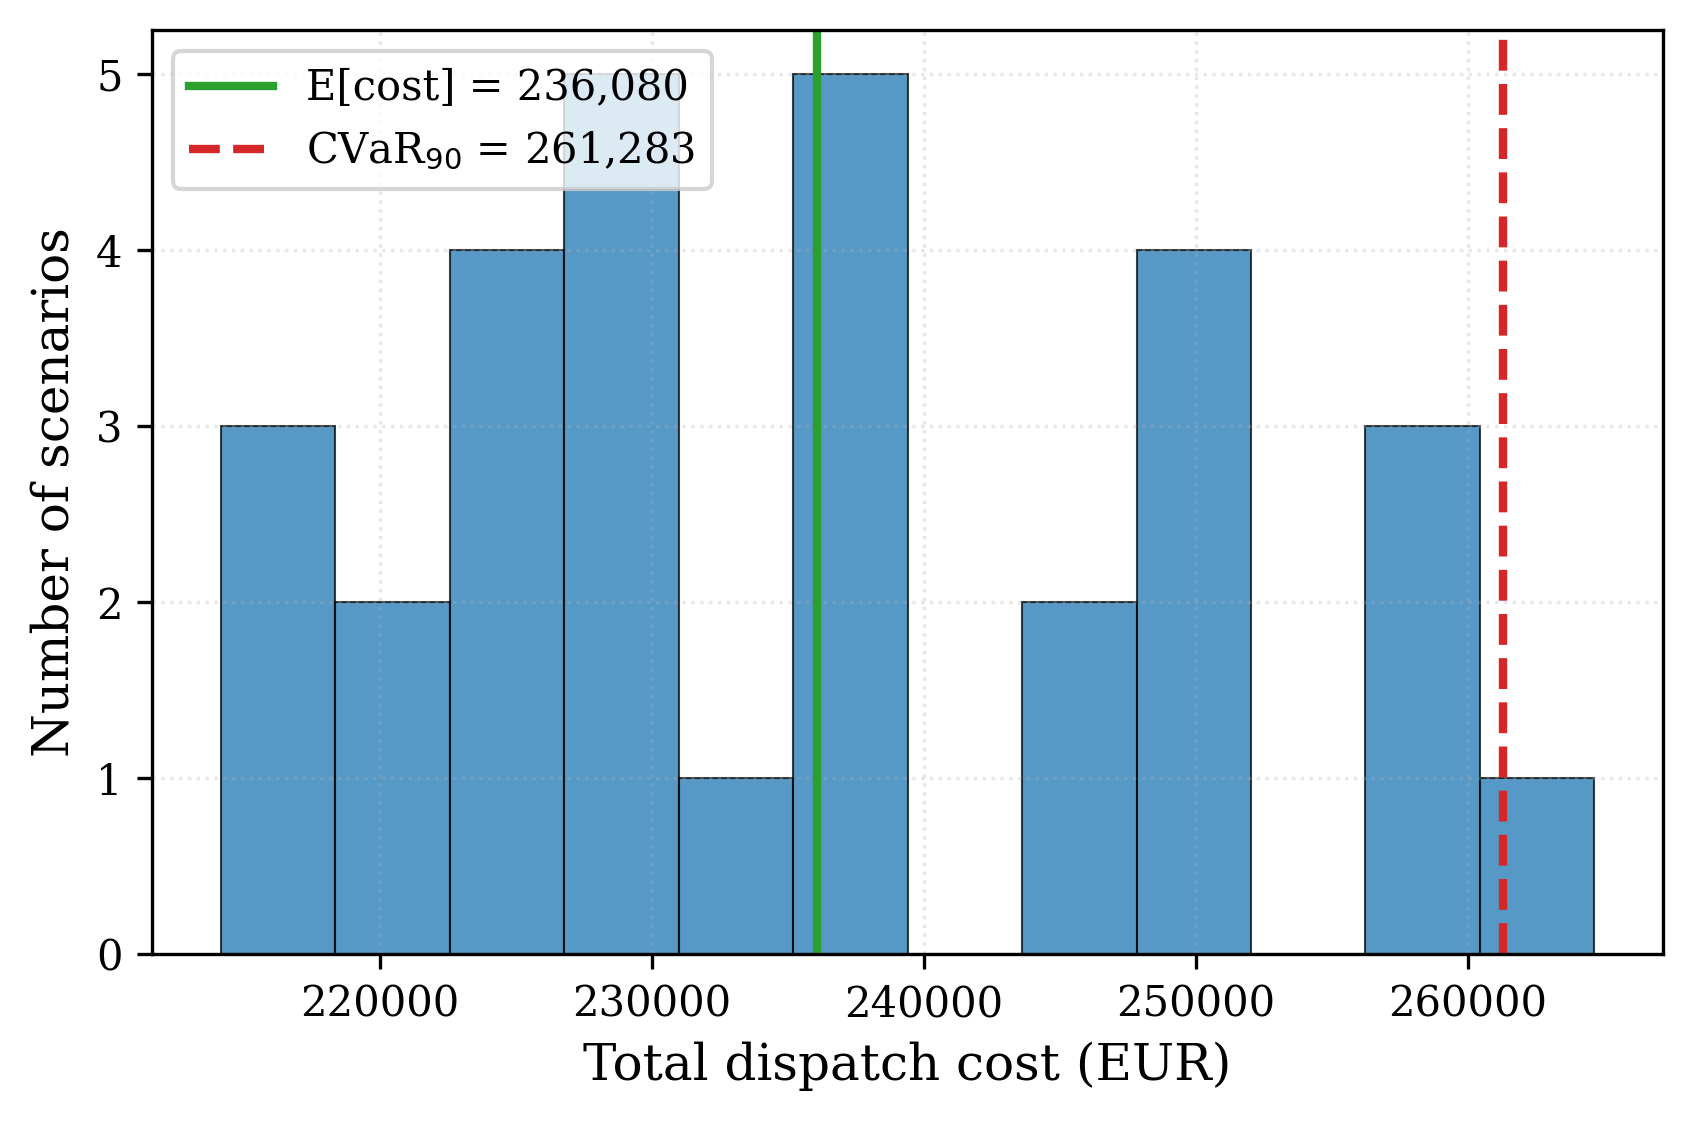
\includegraphics[width=0.7\textwidth]{plots/fig_ml_scenario_costs.png}
    \caption{Dispatch-cost distribution over demand scenarios sampled from the conformal intervals (stochastic SAA on the sample day). The solid line is the expected cost, the dashed line the CVaR$_{90}$; their gap is the tail-risk reserve.}
    \label{fig:scenario_costs}
\end{figure}

\subsection{Julia Technology: Flux.jl and Stochastic Solver}

The LSTM is implemented entirely in Julia using \textbf{Flux.jl} \cite{innes2018flux}, which provides automatic differentiation via Zygote.jl and the Adam optimizer. The full training pipeline --- data preprocessing, sequence batching, gradient computation, early stopping, and conformal calibration --- is implemented in approximately 200 lines of Julia code with no Python dependencies.

The stochastic LOPF module calls \texttt{lopf\_multiperiod} $S$ times in a loop; each call is independent, making the SAA trivially parallelisable. The current implementation is sequential (single-threaded), but parallelisation via Julia's \texttt{Threads.@threads} or distributed computing via \texttt{Distributed.jl} is a straightforward extension.

Table~\ref{tab:julia_packages_full} updates the Julia package list from Chapter~2 to include the packages added for the AI component.

\begin{table}[H]
\centering
\caption{Julia packages used in the full implementation (including AI component)}
\label{tab:julia_packages_full}
\begin{tabular}{lll}
\toprule
\textbf{Package} & \textbf{Purpose} \\
\midrule
JuMP, HiGHS   & LP/MILP modeling and solving \\
PowerModels, Ipopt & AC power flow \\
Flux.jl       & LSTM training (automatic differentiation) \\
Zygote.jl     & Reverse-mode AD backend for Flux \\
Plots.jl, StatsPlots.jl & Visualization \\
CSV, DataFrames & Benchmark result I/O \\
\bottomrule
\end{tabular}
\end{table}


%% ── Chapter 4: Analysis and Discussion ──────────────────────────────────────
\chapter{Analysis and Discussion}
\label{sec:analysis}

This chapter interprets the experimental results of Chapter~\ref{ch:implementation}: why the measured speedups behave as they do across methods and problem sizes, where the Julia implementation does and does not win, and the practical lessons from the port.


\subsection{Why DC PF Speedup Decreases with Network Size}

For small networks (3--10 buses), the Julia speedup is enormous ($\sim$$2$--$6\times10^{4}$) because:
\begin{itemize}
    \item PyPSA's \texttt{lpf()} carries a fixed Python overhead of approximately $120\,\text{ms}$ (DataFrame validation, network state management, pandas operations) regardless of network size.
    \item Julia's DC PF for a 3-bus network completes in $< 0.01\,\text{ms}$ --- effectively instantaneous.
    \item The speedup is dominated by the fixed overhead: $\text{speedup} \approx 120\,\text{ms} / t_\text{Julia}$.
\end{itemize}

These small-network ratios must therefore \emph{not} be read as compute superiority. As the network grows, the sparse linear solve comes to dominate both sides and the ratio collapses toward the true compute-bound figure: $169\times$ at 300 synthetic buses and only $4.7\times$ on the 2{,}869-bus PEGASE network. The honest headline for DC power flow is therefore a low single-digit speedup at scale, not the headline ratio.

\subsection{Why the LOPF Speedup Stays Large at Scale}

Unlike DC power flow, the LOPF speedup does not collapse: it declines only gently with size ($283\times \to 118\times$ on synthetic networks) and stabilises around $58$--$117\times$ on the real IEEE/PEGASE cases. The reason is that for LOPF the dominant cost on the PyPSA side is not a fixed per-call overhead but the \emph{model assembly itself}, which grows with the problem and which Julia performs in compiled code. Three compounding effects explain this:

\begin{enumerate}
    \item \textbf{JuMP model construction efficiency:} JuMP constructs the constraint matrix directly in compiled native code. PyPSA's linopy builds constraints via Python object loops and pandas, with per-constraint overhead that accumulates with problem size.
    \item \textbf{LP matrix sparsity:} For a network with $n$ buses and $|\mathcal{E}|$ lines, the LP has $O(n)$ variables and $O(n + |\mathcal{E}|)$ constraints. JuMP's sparse assembly scales as $O(n + |\mathcal{E}|)$, while linopy's Python loops carry additional interpreter overhead per constraint.
    \item \textbf{Solver parity:} Both implementations use HiGHS as the LP solver, so solver time is identical. The entire measured speedup comes from model-building overhead --- which the multi-period benchmark isolates directly, PyPSA's time staying flat at $\approx 1.14\,\text{s}$ while Julia's grows with the horizon.
\end{enumerate}

\subsection{AC Power Flow: Algorithm vs.\ Language Overhead}
\label{sec:analysis_ac}

The AC power flow benchmark measures a fundamentally different quantity than the DC and LOPF benchmarks. In those cases both implementations execute the same algorithm (sparse linear solve; LP via HiGHS), so the speedup isolates pure language overhead. For AC power flow, the two implementations use different algorithms:

\begin{itemize}
    \item \textbf{Julia (PowerModels.jl + Ipopt):} casts the power flow as a nonlinear optimisation problem and solves it with an interior-point method. Ipopt is a general-purpose NLP solver; its per-iteration cost is higher than Newton--Raphson and it requires more iterations to converge.
    \item \textbf{Python (PyPSA \texttt{pf()}):} applies Newton--Raphson (NR) iteration directly to the power flow mismatch equations. NR typically converges in 3--5 iterations for well-conditioned networks and is computationally efficient for this specific problem structure.
\end{itemize}

At small sizes Julia appears faster ($24.6\times$ at 3 buses), but this is again PyPSA's fixed Python overhead ($\approx 180\,\text{ms}$) masking the actual solve. As the overhead is amortised the comparison reverses: $6.3\times$ at 10 buses, $1.5\times$ at 50 buses, and at 100 buses Julia is about \textbf{twice as slow} as PyPSA ($0.5\times$). This is the honest outcome and the one method where the porting strategy does not pay off. The cause is algorithmic: the Ipopt interior-point solver carries a higher per-iteration cost and more iterations than Newton--Raphson, and because the AC work is dominated by this third-party solver, Julia's compiled model-assembly advantage --- decisive for the LP methods --- has nothing to act on.

The implication is that recovering an AC advantage would require a native Newton--Raphson implementation in Julia (without the Ipopt wrapper), exploiting the specific structure of the power flow equations. Such an implementation is identified as a natural direction for future work (Section~\ref{sec:future}).

\subsection{JIT Compilation Amortization}

Julia's JIT compilation introduces a one-time startup cost (time-to-first-execution, TTFX) of 2--5 seconds per function. For the use cases targeted by this thesis --- large-scale energy system studies where thousands of LP solves are performed per scenario run --- this one-time cost is negligible. PyPSA-Eur, for instance, solves hundreds of LP problems per country-level scenario, making the per-solve LP advantage (tens to a few hundred times, e.g.\ $58\times$ on the 2{,}869-bus PEGASE grid) directly applicable once amortised.

\subsection{Summary of Implementation Challenges}

The three most significant challenges encountered during the porting process are documented here for future reference:

\begin{enumerate}
    \item \textbf{PowerModels.jl data format completeness:} The format requires 15+ mandatory fields per component. Several fields (\texttt{g\_fr}, \texttt{b\_fr}, \texttt{g\_to}, \texttt{b\_to}) are not prominently documented and were discovered by reading the PowerModels.jl source code. Missing any required field produces a \texttt{KeyError} at solve time rather than a meaningful validation message.

    \item \textbf{Per-unit conversion in AC power flow:} PyPSA handles unit conversion transparently at the Python layer. The Julia implementation requires explicit conversion of all quantities. The diagnostic symptom of incorrect conversion is physically unreasonable angles (e.g., $\theta > \pi\,\text{rad}$) without an obvious error message.

    \item \textbf{Susceptance formula for mixed unit systems:} The formula $b = S_\text{base}/x_\text{p.u.}$ gives susceptance in MW/rad when $x$ is in per-unit and the result is used in a physical MW power balance. Using $b = 1/x_\text{p.u.}$ (unitless per-unit susceptance) produces angles that are 100 times smaller than physically correct, causing the optimizer to find trivial but incorrect solutions.
\end{enumerate}


%% ── Chapter 5: Conclusions ──────────────────────────────────────────────────
\chapter{Conclusions and Future Work}
\label{ch:conclusions}

This chapter draws together the findings of the thesis. The first section summarises the key quantitative results established in Chapter~3. The second section states the principal conclusions regarding Julia's viability as a high-performance alternative to Python for power system computation, addressing in turn each research question posed in the Introduction. The final section identifies a structured programme of future work that extends the implemented modules toward a broader Julia-based power system analysis framework.

% ──────────────────────────────────────────────────────────────────────────────
\section{Summary of Results}
% ──────────────────────────────────────────────────────────────────────────────

This thesis implemented and evaluated eight computational contributions: three core power system solvers ported from PyPSA to Julia (DC Power Flow, AC Power Flow, and single-period LOPF), an extension to multi-period LOPF with storage and wind, Unit Commitment (MILP), an LSTM load forecaster with conformal prediction intervals, a scenario-based stochastic LOPF, and a systematic validation campaign on standard IEEE test cases. The key findings are summarised below.

\textbf{Numerical correctness on 3-bus network.}
For the LP-based methods --- single-period LOPF, multi-period LOPF, locational marginal prices, and emission-constrained dispatch --- the Julia and PyPSA results are numerically identical (zero difference in generator dispatch, total cost, and nodal prices). For the power flow modules, active and reactive power flows agree to better than $10^{-3}$, while two quantities differ by a constant scale factor: the DC power flow voltage angles and the transformer branch flow. Both differences trace to a documented per-unit convention difference --- PyPSA normalises branch susceptance by $V_\text{nom}^2$ and the transformer reactance by its own rating $s_\text{nom}$, whereas the present implementation follows the MATPOWER convention of expressing susceptance in MW/rad on the system base. Crucially, these convention differences do not affect any economically meaningful quantity (dispatch, cost, or price), confirming the correctness of the porting.

\textbf{IEEE 14-bus standard test case validation.}
The implementations were additionally validated on the IEEE 14-bus benchmark network \cite{zimmerman2011matpower}. The AC power flow solution matches the MATPOWER reference to within $1.33 \times 10^{-3}$\,p.u.\ in voltage magnitude and $0.017^{\circ}$ in angle. The DC power flow and LOPF solutions from Julia and PyPSA are identical to numerical precision. This confirms that the implementations generalise correctly beyond the construction network.

\textbf{DC Power Flow performance.}
Measured as the noise-robust minimum with threads pinned, Julia's DC power flow speedup falls from $\sim$$6\times10^{4}$ on a 3-bus network to $169\times$ at 300 synthetic buses, and to $4.7\times$ on the 2{,}869-bus PEGASE network. The huge small-network ratios are PyPSA's fixed $\approx 120\,\text{ms}$ Python overhead, not a compute advantage; the honest compute-bound figure at scale is a low single-digit factor.

\textbf{AC Power Flow performance.}
AC power flow is the one method where Julia does \emph{not} hold a consistent advantage. The apparent speedup at small sizes ($24.6\times$ at 3 buses) is again PyPSA's fixed overhead; once amortised, the comparison reverses --- $1.5\times$ at 50 buses and $0.5\times$ at 100 buses, i.e.\ Julia is about twice as slow. The cause is algorithmic: Julia delegates AC power flow to the Ipopt interior-point solver (PowerModels.jl), whose per-iteration cost exceeds PyPSA's specialised Newton--Raphson, and the model-assembly advantage that drives the LP results has nothing to act on when a third-party nonlinear solver dominates.

\textbf{Single-period LOPF performance.}
The Julia LOPF (JuMP + HiGHS) is $118$--$283\times$ faster on synthetic networks and $58$--$117\times$ faster on the standard IEEE/PEGASE cases; on the 2{,}869-bus PEGASE grid PyPSA takes $28.4$\,s against Julia's $0.49$\,s ($58\times$). Since both implementations use the same HiGHS LP solver, the entire speedup comes from JuMP's compiled model assembly versus PyPSA/linopy's Python constraint construction. The speedup declines gently with size but remains large at scale, which is directly applicable to large-scale studies such as PyPSA-Eur.

\textbf{Multi-period LOPF with storage and wind.}
The 24-hour multi-period LOPF with a StorageUnit and variable wind generation was successfully implemented and validated. Both Julia and PyPSA find the same optimal cost of $126{,}790.79\,\text{\euro}$. The LP correctly exploits time-arbitrage: the storage charges at night ($\approx 22\,\text{\euro/MWh}$ round-trip) and discharges at peak to displace expensive backup generation ($50\,\text{\euro/MWh}$). Performance benchmarks over horizons $T \in \{6, 12, 24, 48\}$ hours show Julia achieving $89$--$298\times$ speedups. The PyPSA solve time is nearly constant ($\approx 1.14\,\text{s}$) across all horizons, a direct demonstration that PyPSA's bottleneck is model assembly rather than solving; Julia's solve time scales linearly with $T$, from $3.8$\,ms at $T = 6$ to $12.8$\,ms at $T = 48$.

\textbf{Unit Commitment.}
The MILP Unit Commitment solver was implemented and benchmarked. Julia achieves $17$--$79\times$ speedups over PyPSA across horizons $T \in \{6, 12, 24\}$ and network sizes of 3--30 buses. The speedup is lower than for continuous LOPF because the MILP branch-and-bound search --- executed by the same HiGHS solver in both implementations --- constitutes the dominant cost. LMPs are extracted via LP relaxation with binaries fixed, following the standard electricity market methodology~\cite{oneill2005}.

\textbf{AI component: LSTM forecasting and stochastic dispatch.}
An LSTM load forecaster (Flux.jl, hidden size 64, weekly 168\,h window, 24\,h horizon, residual-to-seasonal-naive target with conformal calibration) was trained and evaluated on \emph{real} German load (OPSD/ENTSO-E) with a strict 60-day out-of-time hold-out, averaged over three seeds. The honest finding is reported as it stands: the LSTM beats the persistence baseline ($+42.7\%$ RMSE skill, $+61.5\%$ with temperature) but \emph{does not} beat the seasonal-naive baseline (MAPE $5.83\%$ with calendar features, $3.67\%$ with idealized temperature, versus $2.77\%$ for seasonal-naive). For aggregate national load the weekly cycle is nearly deterministic, so a learned model adds value only through an exogenous signal; temperature is confirmed to be that decisive lever, closing the gap from $-84\%$ to $-23\%$ RMSE skill.

The contribution of the AI component is therefore not point-forecast accuracy but the \emph{uncertainty quantification} it enables. The conformal intervals are propagated into a scenario-based stochastic LOPF (Sample Average Approximation), which on the demonstration network returns an expected cost, a worst-case CVaR$_{90}$, and a cost spread ($\sigma$). The gap between expected and worst-case cost ($\approx 13\%$) is the reserve a risk-averse operator must budget for the worst $10\%$ of demand outcomes --- a decision-relevant risk measure that no deterministic dispatch, however accurate its point forecast, can provide.

This AI component is presented as a methodological contribution rather than a production forecaster. Its honest limitation --- a neural forecaster that loses to a trivial seasonal baseline on point accuracy --- is itself an informative result: it locates the value of machine learning in this domain in calibrated uncertainty and weather-informed features rather than in architecture alone, and it motivates the future work in Section~\ref{sec:future}.

% ──────────────────────────────────────────────────────────────────────────────
\section{Conclusions}
% ──────────────────────────────────────────────────────────────────────────────

The experimental results demonstrate that porting PyPSA's core algorithms to Julia is both feasible and highly beneficial. The main conclusions are:

\begin{enumerate}
    \item \textbf{Julia is a viable replacement for Python in power system computation.}
    The mathematical formulations translate directly from PyPSA's Python code, and the Julia ecosystem (JuMP, HiGHS, PowerModels.jl) provides mature, well-maintained tools for every required component. Validation on both a custom 3-bus network and the standard IEEE 14-bus case confirms numerical equivalence.

    \item \textbf{The performance advantage is largest for LP-based optimisation.}
    The LP-based methods (single- and multi-period LOPF, unit commitment) are tens to a few hundred times faster, and the advantage persists at scale ($58\times$ for LOPF on the 2{,}869-bus PEGASE grid, where PyPSA takes $28$\,s and Julia under $0.5$\,s). Because both sides call the same HiGHS solver, this gain is entirely the compiled model-assembly layer --- making Julia particularly valuable for iterative large-scale studies such as PyPSA-Eur.

    \item \textbf{Multi-period optimisation with storage scales naturally.}
    Extending the single-period LOPF to 24 time periods with a StorageUnit required only incremental additions to the JuMP model --- SOC dynamics, charge/discharge variables, and a cyclicity constraint. The Julia implementation produces results identical to PyPSA, confirming that the time-coupling constraints are correctly formulated.

    \item \textbf{Algorithm choice matters more than language for AC power flow.}
    AC power flow is the honest exception: Julia is competitive only at small sizes and becomes about twice as slow as PyPSA at 100 buses, because it delegates to the Ipopt interior-point solver while PyPSA uses a specialised Newton--Raphson iteration. The compiled model-assembly advantage that drives the LP speedups does not apply when a third-party nonlinear solver dominates the work. A native Newton--Raphson implementation in Julia would be required to recover an advantage here.

    \item \textbf{JIT warmup is not a practical barrier.}
    For realistic use cases --- time-series analysis, scenario sweeps, iterative optimisation --- functions are invoked thousands of times, making the one-time JIT compilation cost ($2$--$5\,\text{s}$) negligible. The benchmarks in this thesis measure steady-state (post-warmup) performance, which is the relevant metric for production use.

    \item \textbf{The existing Julia power system landscape has a gap.}
    As documented in the literature review (Chapter~\ref{ch:litreview}), no actively maintained, self-contained Julia reimplementation of PyPSA exists. PSA.jl and EnergyModels.jl were abandoned years ago; PowerModels.jl and PowerSimulations.jl follow independent architectures. This thesis provides a validated starting point for filling that gap.

    \item \textbf{AI-assisted dispatch quantifies risk, even when the forecaster does not win on accuracy.}
    On real load data the LSTM does not beat the seasonal-naive baseline on point accuracy --- a result reported honestly. Its value lies elsewhere: the conformal prediction framework provides distribution-free $90\%$-coverage intervals with no assumption on the residual distribution, and propagating these into the stochastic SAA gives operators a CVaR$_{90}$ tail-risk estimate that is inaccessible to any deterministic formulation, however accurate its point forecast. The AI component thus demonstrates that the value of machine learning in this pipeline is calibrated uncertainty quantification feeding risk-aware dispatch, not raw forecast accuracy.
\end{enumerate}

% ──────────────────────────────────────────────────────────────────────────────
\section{Future Work}
\label{sec:future}
% ──────────────────────────────────────────────────────────────────────────────

This thesis provides a foundation for a broader Julia-based power system analysis framework. Several concrete directions for future work are identified.

\textbf{Native Newton--Raphson AC power flow.}
The current AC power flow implementation delegates to Ipopt, which makes Julia slower than PyPSA's specialised Newton--Raphson at 100 buses. Implementing a direct Newton--Raphson solver in Julia --- building and factorising the Jacobian matrix natively --- would remove this algorithmic penalty and is the most impactful single improvement, as it is the only method where the present implementation does not already outperform PyPSA.

\textbf{Parallel stochastic LOPF.}
The SAA implemented in Section~\ref{sec:ai_component} solves $S$ independent LOPFs sequentially. Each scenario solve is fully independent, making the SAA embarrassingly parallel. Exploiting \texttt{Threads.@threads} or \texttt{Distributed.pmap} in Julia would reduce stochastic LOPF wall-clock time by a factor of $S$ on a multi-core machine, enabling real-time stochastic dispatch.

\textbf{Numerical validation on larger standard cases.}
Performance was already benchmarked on the IEEE 118/300 and PEGASE 1354/2869 networks, and numerical validation against PyPSA was performed on the 3-bus and IEEE 14-bus cases. A natural extension is a full variable-by-variable numerical validation against PyPSA on the larger PEGASE cases, and eventually on a subset of the PyPSA-Eur European transmission network \cite{horsch2018pypsa_eur}, to extend the equivalence guarantee to real-world problem sizes.

\textbf{Weather-informed and residual forecasting.}
The evaluation showed that the LSTM matches the seasonal-naive baseline only with idealized (perfect-foresight) temperature. Coupling the forecaster to an actual numerical weather prediction feed, and combining it with the strong seasonal-naive baseline in an explicit residual model, is the most promising route to a forecaster that genuinely improves on the naive baselines on real out-of-time data.

\textbf{Security-constrained OPF.}
Adding N-1 contingency constraints for transmission line or generator outages would produce a security-constrained LOPF (SCLOPF), which is a standard requirement for transmission system operator studies.

\textbf{Capacity expansion planning.}
Extending the multi-period LOPF with investment variables (\texttt{p\_nom\_extendable}) would enable greenfield or retrofit generation planning studies, equivalent to PyPSA's capacity expansion mode.

\textbf{PyPSA data format interoperability.}
Developing a Julia reader for PyPSA's native netCDF/HDF5 network format would enable seamless use of existing PyPSA-Eur model files in the Julia solvers, without requiring manual data conversion.

The results of this thesis demonstrate that a Julia-based power system analysis framework can deliver order-of-magnitude performance improvements over Python while maintaining numerical equivalence with PyPSA, and that integrating a data-driven forecasting layer enables uncertainty-aware, risk-quantified dispatch decisions that are inaccessible to deterministic formulations.


%% ── Bibliography ────────────────────────────────────────────────────────────
\printbibliography[heading=bibintoc]

\end{document}
